\documentclass[titlepage]{article}
\usepackage{babel}
\usepackage{amsmath}
\usepackage{amssymb}
\usepackage{amsthm}
\usepackage{multicol} %spalten in seite
\usepackage{graphicx} %bilder einfügen
\usepackage{tabto} %tabulator mit \tab
\usepackage{hyperref}
\usepackage{bbm}
\usepackage{tikz}
\usetikzlibrary{shapes.geometric}
 \usepackage{bbold}
\usepackage[T1]{fontenc}
\usepackage{mathrsfs}  
\usepackage[utf8]{inputenc}
\usepackage{listings} %quellcode
\pagestyle{plain}
\usepackage{varwidth}
\pagenumbering{arabic}
\renewcommand{\arraystretch}{1.3} %vertikaler abstand von tabellen
\newcommand{\n}{\newline}
\usepackage[left=20mm, right=17mm, top=25mm, bottom=30mm, paper=a4paper]{geometry}
\renewcommand{\contentsname}{Inhaltsverzeichnis}

\newcommand{\K}{\mathbb{K}}
\newcommand{\C}{\mathbb{C}}
\newcommand{\N}{\mathbb{N}}
\newcommand{\Q}{\mathbb{Q}}
\newcommand{\R}{\mathbb{R}}
\newcommand{\1}{\mathbb{1}}
\newcommand{\0}{\mathbb{0}}
\newcommand{\Z}{\mathbb{Z}}
\newcommand{\T}{\mathbb{T}}
\newcommand{\isom}{\overset{\cong}{\rightarrow}}

\newcommand{\vecD}[3]{\left(\begin{smallmatrix}#1\\#2\\#3\end{smallmatrix}\right)}
\newcommand{\matrixZ}[4]{\begin{pmatrix}#1&#2\\#3&#4\end{pmatrix}}
\newcommand{\detZ}[4]{\begin{vmatrix}#1&#2\\#3&#4\end{vmatrix}}
\newcommand{\smallMatrixZ}[4]{\left(\begin{smallmatrix}#1&#2\\#3&#4\end{smallmatrix}\right)}
\newcommand{\smallDetZ}[4]{\left|\begin{smallmatrix}#1&#2\\#3&#4\end{smallmatrix}\right|}
\newcommand{\vecZ}[2]{\left(\begin{smallmatrix}#1\\#2\end{smallmatrix}\right)}
\newcommand{\detD}[9]{\begin{vmatrix}#1&#2&#3\\#4&#5&#6\\#7&#8&#9\end{vmatrix}}

\newcommand\Umbruch[2][13.5cm]{\begin{varwidth}{#1}\centering#2\end{varwidth}}

	
\begin{document}
	
	\begin{center}
		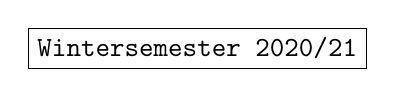
\begin{tikzpicture}
			\draw (0,0) node[draw, rectangle]{\texttt{Wintersemester 2020/21}};
		\end{tikzpicture}
		\hrulefill\\
		\begin{center}
			\quad\\
			\LARGE Definitionssammlung Wintersemester 2020 \normalsize\\
		\end{center}
		\hrulefill
		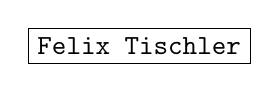
\begin{tikzpicture}
			\draw (0,0) node[draw, rectangle]{\texttt{Felix Tischler}};
		\end{tikzpicture}
		\date{\today}
	\end{center}
	\tableofcontents
	
	\part*{Lineare Algebra}
		\section{Grundlagen}
			\subsection{Logik}
				\subsubsection{Aussagen}
					\begin{itemize}
						\item Negation: $\neg P$ "nicht P"
						\item Konjunktion: $P\wedge Q$ "P und Q"
						\item Disjunktion: $P\vee Q$ "P oder Q"
						\item Implikation: $P\Rightarrow Q$ "Wenn P, dann Q"
						\item Äquivalenz: $P\Leftrightarrow Q$ "P genau dann wenn Q"
					\end{itemize}
				\subsubsection{gleichbedeutende Aussagen}
					\begin{itemize}
						\item $P\Leftrightarrow \neg\neg P$
						\item $\neg(P\Rightarrow Q)\Leftrightarrow P\wedge (\neg Q)$
						\item $\neg(P\wedge Q)\Leftrightarrow(\neg P)\vee(\neg Q)$
						\item $\neg(P\vee Q)\Leftrightarrow(\neg P)\wedge(\neg Q)$
					\end{itemize}
				\subsubsection{Aussageformen und Quantoren}
					\begin{itemize}
						\item Aussagenlogik erweitert zur \textbf{Prädikatenlogik}
						\item n-stelliges \textbf{Prädikat} (auch \textbf{Aussageform}) ist Ausdruck von n Variablen, welcher durch einsetzten von konkreten Werten Aussage wird
						\item $\forall$ "für alle"
						\item $\exists$ "für mindestens eins"
						\item $\exists$! "es gibt genau ein"
						\item Der Gültigkeitsbereich von Quantoren sollte im Zweifel geklammert werden
					\end{itemize}
				\subsubsection{Beweisstrategien}
					Seien P,Q Aussagen bzw. Prädikate.
					\begin{itemize}
						\item \textbf{Direkter Beweis}: \underline{Unter der Voraussetzung}, dass P gilt ist zz. das Q gilt.
						\item \textbf{Beweis durch Kontraposition}: Ersetze $P\Rightarrow Q$ durch $\neg Q\Rightarrow\neg P$ und beweise dies direkt. Aus Voraussetzung, das Q nicht gilt leite man her das P nicht gilt.
						\item \textbf{Widerspruchsbeweis}: Ersetze $P\Rightarrow Q$ durch $\neg(P\wedge\neg Q)$. Somit weist man nach, dass nicht gleichzeitig P und Q falsch sein kann. Anders gesagt: Man setzt zunächst P voraus; dann nimmt man an, das Q falsch ist, und leitet aus der Voraussetzung und der Annahme einen Widerspruch her.
					\end{itemize}
			\subsection{Mengen}
				\subsubsection{Extensionalitätsaxiom}
					Zwei Mengen sind \textbf{gleich} gdw. sie die gleichen Elemente haben.
				\subsubsection{Teilmenge}
					\begin{itemize}
						\item Eine Menge N heißt Teilmenge einer Menge M gdw. jedes Element von N auch ein Element von M ist.
						\item Bezeichnung: $N\subseteq M$ bzw. $N\subset M$
						\item \textbf{echte Teilmenge}: $N\subsetneq M$, heißt $(N\subset M)\wedge(N\neq M)$
						\item $M=N\Longleftrightarrow(M\subseteq N\wedge N\subseteq M)$
					\end{itemize}
				\subsubsection{Schnitt, Vereinigung und Durchschnitt}
					\begin{itemize}
						\item \textbf{Schnitt} (auch \textbf{Durchschnitt} oder auch \textbf{Schnittmenge}) $M\cap N$ besteht aus allen Elementen die in M und N sind
						\item $M\cap N:=\{x\mid(x\in M)\wedge(x\in N)\}$\\
						\item \textbf{Differenz} $M\textbackslash N$ besteht aus alle Elementen, die in M und nicht in N sind
						\item $M \textbackslash N:=\{x\in M\mid x\notin N\}$\\
						\item \textbf{Vereinigung} $M\cup N$ besteht aus allen Elementen die in M sind und aus alle die in N sind (basiert auf \textbf{Viereinigungsaxiom})
						\item $M \cup N:=\{x\mid(x\in M)\vee(c\in N)\}$
					\end{itemize}
				\subsubsection{Angaben von Mengen}
					\begin{itemize}
						\item z.B. $M:=\{1,2,3,4,5\}$
						\item z.B. $\Z:=\{...,-2,-1,0,1,2,...\}$
						\item Aussonderungsaxiom
						\item Ersetzungsaxiom
					\end{itemize}
				\subsubsection{Aussonderungsaxiom}
					\begin{itemize}
						\item Ist M eine Menge und P eine 1-stellige Aussageform, so ist die Gesamtheit $\{x\in M\mid P(x)\}$ der Elemente von M, durch die P wahr wird, eine Menge
						\item z.B. $M:=\{m\in\Z\mid\exists k\in\N:k^2=m\}$
					\end{itemize}
				\subsubsection{Ersetzungsaxiom}
					\begin{itemize}
						\item Ersetzt man jedes Element einer gegebenen Menge durch ein "Objekt unserer Anschauung oder unseres Denkens", so entsteht wieder eine Menge
						\item z.B. $\{n^2\mid n\in\Z\}$
					\end{itemize}
				\subsubsection{Notation von Mengen}
					\begin{itemize}
						\item $\underset{A\in X}{\text{\LARGE $\cup$}}A:=\{x\mid\exists A\in X:x\in A\}$ und $\underset{A\in X}{\text{\LARGE $\cap$}}A:=\{x\mid\forall A\in X:x\in A\}$
						\item $\emptyset$, \{\} die \textbf{leere Menge}, ihre Existenz wir im \textbf{Leermengenaxiom} gefordert
						\item $\N$ Menge der natürlichen Zahlen. Die Existenz von $\N$ folgt aus dem \textbf{Unendlichkeitsaxiom}
						\item $\N^*$ Menge der natürlichen Zahlen ohne 0 (Menge der pos. nat. Zahlen)
						\item $\Z$ Menge der ganzen Zahlen
						\item $\Q$ Menge der rationalen Zahlen
						\item $\R$ Menge der reellen Zahlen
						\item $\Q_{>0}$ Menge der pos. rat. Zahlen (Analog $\Q_{\geq0},\R_{<0}$ etc.)
						\item $\C$ Menge der komplexen Zahlen.
					\end{itemize}
				\subsubsection{Intervallschreibweise}
					Für $a,b\in\R,a\le b$, bezeichnet man $[a,b]:=\{x\in\R\mid a\le x\le b\}, ]a,b]:=\{x\in\R\mid a<x\le b\}$, analog $[a,b[$ und $]a,b[$, ferner $]-\infty,a]:=\{x\in\R\mid x\le a\}$ etc.
				\subsubsection{Kardinalität bzw. Mächtigkeit}
					\begin{itemize}
						\item Die Anzahl der Elemente einer endlichen Menge z.b. M
						\item Notation: $\mid M\mid$
					\end{itemize}
				\subsubsection{kartesische Produkt bzw. direkte Produkt}
				Seien $M,N$ Mengen, ihr kartesisches Produkt ist:
					\begin{itemize}
						\item Alle \textbf{geordnete Paare} $(m,n)$ mit $m\in M$ und $n\in N$
						\item $M\times N:=\{(m,n)\mid m\in M,n\in N\}$
						\item $(1,2)\neq(2,1)$
						\item Analog bezeichnet man Ausdrücke der Form $(a,b,c)$ \textbf{Tripel} und $(x_1,...,x_n)$ als n-\textbf{Tupel}
						\item Für $M_1,...,M_n$ Mengen, ist ihr kartesisches Produkt $M_1\times...\times M_n:=\{(m_1,...,m_n)\mid m_1\in M_1,...,m_n\in M_n\}$
						\item Statt $\underbrace{M\times,...,\times M}_{n-mal}$ schreibt man $M^n$
					\end{itemize}
				\subsubsection{Potenzmenge}
					Sei M eine Menge.
					\begin{itemize}
						\item Die Gesamtheit der Teilmengen von M bildet die \textbf{Potenzmenge}
						\item $\mathscr{P}(M):=\{T\mid T\subseteq M\}$
						\item Z.B. $\mathscr{P}(\{1,2,3\}):=\{\emptyset,\{1\},\{2\},\{3\},\{1,2\},\{1,3\},\{2,3\},\{1,2,3\}\}$
						\item Ist M endlich, so gilt $\mid\mathscr{P}(M)\mid=2^{\mid M\mid}$
					\end{itemize}
				\subsubsection{Klasse}
					\begin{itemize}
						\item P 1-stelliges Prädikat: $\{x\mid P(x)\}$ ist eine \textbf{Klasse}
						\item Klasse x heißt \textbf{Menge} gdw. es eine Klasse y mit $x\in y$ gibt.
						\item Eine Klasse die keine Menge ist heißt \textbf{echte Klasse}
						\item $R:=\{x\mid x\notin x\}$ ergibt keinen Widerspruch: $R$ ist eine echte Klasse, die x in der Definition von $R$ sind aber Mengen, also ist $R\notin R$ unproblematisch
					\end{itemize}
				\subsubsection{Abbildung bzw. Funktion}
					Seien M (\textbf{Definitionsmenge}),N (\textbf{Zielmenge}) Mengen.
					\begin{itemize}
						\item \textbf{Abbildung} $f$ ordnet jedem Element $m\in M$ ein Element von N zu, welches als $f(m)$ notiert wird
						\item Notation: $f:M\rightarrow N$
						\item $N^M$ oder Abb(M,N) ist \textbf{Gesamtheit aller Abbildungen} von M nach N und eine Menge
						\item Für $f,g\in N^M\text{ gilt }f=g\Longleftrightarrow\forall m\in M:f(m)=g(m)$
						\item Sind M,N endlich, gilt: $\mid N^M\mid=\mid N\mid^{\mid M\mid}$
					\end{itemize}
					Alternative Definition: Seien M,N Mengen.
					\begin{itemize}
						\item Eine Teilmenge $f\subset M\times N$ ist eine \textbf{Abbildung} von M nach N gdw. $\forall m\in M: \exists!n\in N:(m,n)\in f$
						\item Statt $(m,n)\in f$ schreibt man $f(m)=n$
					\end{itemize}
			\subsection{Summen- und Produktzeichen}
				Sei $n\in N$ und $a_1,...,a_n\in\R$.
				\begin{itemize}
					\item \textbf{Summe} der $a_1,...,a_n$ ist $\sum\limits^n_{i=1}a_i:=a_1+...+a_n$
					\item \textbf{Produkt} der $a_1,...,a_n$ ist $\prod\limits^n_{i=1}a_i:=a_1\cdot...\cdot a_n$
					\item $\sum\limits^0_{i=1}a_i:=0$ bzw. $\prod\limits^0_{i=1}a_i:=1$
				\end{itemize}
				Für $n\in\N^*$:
				\begin{itemize}
					\item $\sum\limits^n_{i=1}a_i:=\left(\sum\limits^{n-1}_{i=1}a_i\right)+a_n$
					\item $\prod\limits^n_{i=1}a_i:=\left(\prod\limits^{n-1}_{i=1}a_i\right)\cdot a_n$
				\end{itemize}
		\section{Ringe und Körper}
			\subsection{innere Verknüpfung}
				\begin{itemize}
					\item \textbf{Innere Verknüpfung} ist eine Abbildung $M\times M\rightarrow M$
					\item statt $f(a,b)$ wird eines von vielen möglichen \textbf{Verknüpfungssymbolen} verwendet
					\item Z.B. $a*b,a\otimes b$ etc.
					\item Ist die Menge endlich, so lässt sich die Verknüpfung durch eine Verknüpfungstafel angeben 
				\end{itemize}
			\subsection{Ring}
				\begin{itemize}
					\item Ein \textbf{Ring} $(R,+,\cdot,0,1)$ ist eine Menge R zusammen mit zwei inneren Verknüpfungen + und $\cdot$, einem \textbf{Nullelement} $0\in R$ und einem \textbf{Einselement} $1\in R$, so dass die \textbf{Ringaxiome} erfüllt sind.
				\end{itemize}
				\subsubsection{Ringaxiome}
				Sei R ein Ring $(R,+,\cdot,0,1)$.
					\begin{itemize}
						\item Kommutativität von $+$: $\forall x,y\in R:x+y=y+x$
						\item Assoziativität: $\forall x,y,z\in R:(x\cdot y)\cdot z=x\cdot(y\cdot z)$ und $(x+y)+z=x+(y+z)$
						\item Distributivität: $\forall x,y,z\in R:(x+y)\cdot z=x\cdot z+y\cdot z$ und $x\cdot(y+z)=x\cdot y+x\cdot z$
						\item Neutrale Elemente: $\forall x\in R:x+0=x$ und $x\cdot 1=x$
						\item Negation: $\forall x\in R:\exists-x\in R:x+(-x)=0$; $-x$ ist das \textbf{additive Inverse} von $x$\\
						\item statt $a+(-b)$ schreibt man $a-b$ für alle $a,b\in R$
						\item den Multiplikationspunkt lässt man meist weg
						\item $R^*:=R\textbackslash\{0\}$
						\item ein Ring R ist \textbf{kommutativ} gdw. $\forall x,y\in R:x\cdot y=y\cdot x$
					\end{itemize}
			\subsection{Körper}
				\begin{itemize}
					\item Ein Ring R heißt \textbf{Körper}, gdw. $1\neq0$ und $\forall x\in R^*:\exists x^{-1}\in R:xx^{-1}=x^{-1}x=1$; $x^{-1}$ ist das \textbf{multiplikative Inverse} von x
					\item Die Ringaxiome zusammen mit der Kommutativität von $\cdot$ und der Existenz der multiplikativen Inversen nennt man \textbf{Körperaxiome}
				\end{itemize}
			\subsection{nützliches zu Ringen}
			Sei R ein Ring.
				\begin{itemize}
					\item Kürzungsregel: $\forall x,y,z\in R:(x+z=y+z\Rightarrow x=y)$\\
					Ist R ein Körper, so auch $\forall x,y,z\in R,z\neq0:(xz=yx\Rightarrow x=y)$
					\item Eindeutigkeit der Einselement: $\forall x\in R:(\forall y\in R:y\cdot x=x\cdot y=y)\Rightarrow x=1$
					\item Eindeutigkeit des Nullelements: $\forall x\in R:(\exists y\in R:y+x=y)\Rightarrow x=0$\\
					Ist R ein Körper, so auch $\forall x\in R:(\exists y\in R^*:yx=y)\Rightarrow x=1$
					\item $\forall x\in R:-(-x)=x$\\
					Ist R ein Körper, so auch $\forall x\in R^*:(x^{-1})^{-1}=x$
					\item $\forall x\in R:0\cdot x=0$
					\item $\forall x\in R:(-1)\cdot x=-x$
				\end{itemize}
			\subsection{Restklassenringe, Relation}
				Sei X eine Menge oder Eine Klasse.
					\begin{itemize}
						\item (binäre bzw. zweistellige) \textbf{Relation} auf X ist eine Abbildung $X\times X\rightarrow\{W,F\}$\\
						anders gesagt: eine auf X beschränkte zweistellige Aussageform
						\item Sind $x,y\in X$, Notation z.B.: $x\sim y,x\sim_Ry,x\equiv y, x\cong y$
						\item Relation kann als Teilmenge betrachtet werden: $\{(x,y)\in X\times X\mid x\sim y\}$\\
						\item \textbf{Reflexiv}, wenn: $\forall x\in X:x\sim x$
						\item \textbf{Symmetrisch}, wenn: $\forall x,y\in X:x\sim y\Longleftrightarrow y\sim x$
						\item \textbf{transitiv}, wenn: $\forall x,y,z\in X:$ Wenn $x\sim y$ und $y\sim z$, dann $x\sim z$
					\end{itemize}
				\subsubsection{Äquivalenzrelation}
					\begin{itemize}
						\item Ist eine reflexive symmetrische transitive Relation
					\end{itemize}
				\subsubsection{Ordnungsrelation}
					\begin{itemize}
						\item Weder reflexiv noch symmetrisch, nur transitiv
					\end{itemize}
				\subsubsection{kongruent, modulo}
					Sei R ein kommutativer Ring.
					\begin{itemize}
						\item $\forall a,v\in R:a\mid b:\Leftrightarrow \exists c\in R:b=a\cdot c$, das heißt "a \textbf{teilt} b"
					\end{itemize}
					Sei $n\in R^*$.
					\begin{itemize}
						\item $\forall a,b\in R:a\equiv_nb:\Leftrightarrow n\mid(b-a)$, das heißt a ist \textbf{kongruent} zu b \textbf{modulo} n
						\item $a\equiv b\,(mod\,n)\Leftrightarrow a\,(mod\,n)\equiv b\,(mod\,n)$
					\end{itemize}
				\subsubsection{Äquivalenzklasse, Repräsentant}
					Sei $\sim$ eine Äquivalenzrelation auf der Menge X und $y\in X$
					\begin{itemize}
						\item \textbf{Äquivalenzklasse} von y ist: $[y]:=[y]_\sim:=\{x\in X\mid x\sim y\}$
						\item Ist K eine Äquivalenzklasse und $x\in K$, so heißt x ein \textbf{Repräsentant}
					\end{itemize}
					Wegen Reflexivität gilt $\forall x\in X:x\in [x]$. Außerdem sind für $x,y\in X$ die folgenden drei Aussagen sind gleichbedeutend:
					\begin{enumerate}
						\item $x\sim y$
						\item $[x]\cap [y]\neq\emptyset$
						\item $[x]=[y]$
					\end{enumerate}
				\subsubsection{Restklassenring}
					Sei R ein kommutativer Ring und $n\in R^*$.
					\begin{itemize}
						\item Betrachte die durch $\forall x,y\in R$ durch $x\equiv_ny$ gegebene Äquivalenzrelation.
						\item und definiere $R/_{n}R:=\{[x]\mid x\in R\}$\\
						\item Für $x,y\in R$ sind durch $[x]+[y]:=[x+y]$ und $[x]\cdot[y]:=[x\cdot y]$ zwei innere Verknüpfungen auf $R/_nR$ definiert
						\item Durch diese beiden inneren Verknüpfungen wird $R/_nR$ zu einem kommutativen Ring, dem so genannten \textbf{Restklassenring} von R modulo n\\
					\end{itemize}
				\subsubsection{wohldefiniert}
					\begin{itemize}
						\item unabhängig von der Wahl der Repräsentanten
					\end{itemize}
				\subsubsection{alternierende Quersumme}
					Sei beispielsweise $x\in\N$ mit $z_k,z_{k-1},...,z_0\in\{0,...,9\}$
					\begin{itemize}
						\item \textbf{alternierende Quersumme}: $z_0-z_1+z_2-z_3+z_4-...\pm z_k$
					\end{itemize}
				%\subsubsection{Chinesischer Restsatz}
				\subsubsection{Primzahl}
					\begin{itemize}
						\item $n\in\N^*$ heißt \textbf{Primzahl} gdw. $n\nmid1$ und $\forall a,b\in\Z:n\mid a\cdot b\Rightarrow(n\mid a)\vee(n\mid b)$
						\item Begriff aus der Schule ("n heißt prim gdw. n sich nicht als Produkt zweier von 1 verschiedener nat. Zahlen schreiben lässt") heißt in der Algebra \textbf{irreduzibel}
					\end{itemize}
			\subsection{Komplexe Zahlen}
				\begin{itemize}
					\item \textbf{imaginäre Einheit}: $\mathrm{i}$
					\item $\mathrm{i}^2=-1$
				\end{itemize}
				\subsubsection{Realteil, Imaginärteil}
					\begin{itemize}
						\item $\C:=\{a+b\mathrm{i}\mid a,b\in\R\}$ ist die Menge der \textbf{komplexen Zahlen}
						\item Der \textbf{Realteil} von $z=a+b\mathrm{i}\in\C$ ist $Re(z):=a\in\R$
						\item Der \textbf{Imaginärteil} ist $Im(z):=b\in\R$
					\end{itemize}
				\subsubsection{Rechenregeln}
					\begin{itemize}
						\item Für $a\in\R_{>0}$ setzt man $\sqrt{-a}:=\mathrm{i}\sqrt{a}$
						\item $z_1+z_2=(a_1+a_2)+(b_1+b_2)\mathrm{i}$
						\item $z_1\cdot z_2=(a_1a_2-b_1b_2)+(a_1b_2-a_2b_1)\mathrm{i}$
						\item Falls $a_2+b_2\mathrm{i}\neq0:\frac{z_1}{z_2}=\frac{a_1a_2+b_1b_2}{a_2^2+b_2^2}+\frac{a_2b_1-a_1b_2}{a_2^2+b_2^2}$
					\end{itemize}
				\subsubsection{konjugiert komplexe Zahl}
					\begin{itemize}
						\item Für $z=a+b\mathrm{i}\in\C$ mit $a,b\in\R$ ist $\bar z:=a-b\mathrm{i}\in\C$ die \textbf{konjugierte komplexe Zahl}
					\end{itemize}
				\subsubsection{Betrag}
					\begin{itemize}
						\item $\mid z\mid:=\sqrt{z\cdot z}=\sqrt{a^2+b^2}\in\R_{\ge0}$ ist der \textbf{Betrag} von z\\
					\end{itemize}
					Weil stets $a^2+b^2\in\R_{\ge0}$, ist $\mid z\mid\in\R_{\ge0}$. Ferner ist $\mid z\mid=0\Longleftrightarrow z=0$
					\begin{itemize}
						\item Divisionsregel: $\frac{z_1}{z_2}=\frac{z_1\bar z_2}{z_2\bar z_2}=\frac{z_1\bar z_2}{\mid z_2\mid^2}$
					\end{itemize}
				\subsubsection{Fundamentalsatz der Algebra}
				\begin{itemize}
					\item Jedes Polynom vom Grad $\ge1$ mit Koeffizienten aus $\C$ hat mindestens eine Nullstelle in $\C$
				\end{itemize}
				\subsubsection{Die Gaußsche Zahlenebene bzw. Arganddiagramm}
					\begin{itemize}
						\item $\C$ mit der Ebene $\R^2$ identifiziert, indem man $a+b\mathrm{i}\in\C$ als $(a,b)\in\R$ darstellt. 
					\end{itemize}
				\subsubsection{Argument}
					Sei $z=a+b\mathrm{i}\in\C$. Seien $(r,\varphi)$ die Polarkoordinaten (Bogenmaß) des Punkts $(a,b)\in\R^2$, also $r\ge0$ und $a=r\cos(\varphi),b=r\sin(\varphi)$. \\\\Dann $z=a+b\mathrm{i}=r(\cos(\varphi)+\mathrm{i}\sin(\varphi))$\\
					\\Nach Satz des Pythagoras: $r^2=a^2+b^2$, also $r=\mid z\mid$
					\begin{itemize}
						\item Man nennt $\varphi$ das \textbf{Argument} $arg(z)$ von $z$
						\item verschiedene Konventionen: $\varphi\in]-\pi,\pi]$ oder $\varphi\in[0,2\pi[$
					\end{itemize}
				\subsubsection{Polardarstellung bzw. trigonometrische Darstellung}
					\begin{itemize}
						\item $z=r\cdot(cos\varphi+\mathrm{i}\sin\varphi)$
					\end{itemize}
				\subsubsection{Standarddarstellung bzw. kartesische Darstellung}
					\begin{itemize}
						\item $z=a+b\mathrm{i}$
					\end{itemize}
				\subsection{Addition, komplexe Konjugation, etc.}
					\begin{itemize}
						\item \textbf{Addition} in $\C$ entspricht Vektoraddition in $\R^2$
						\item \textbf{Komplexe Konjugation} ist die Spiegelung an der reellen Achse
						\item \textbf{Dreiecksgleichung}: Für $z_1,z_2\in\C$ gilt $\mid z_1+z_2\mid\,\le\,\mid z_1\mid+\mid z_2\mid$
					\end{itemize}
				\subsubsection{Eine paar Sätze zum rechnen in Polarkoordinaten}
					Addition und Konjugtion sind in der Standartdarstellung leicht, Multiplikation oder Wurzelziehen hingegen schwer. Zwar ist Addition in Polarkoordinaten schwer, aber Konjungtion ist leicht: Weil Kojungtion die Spiegelung an der reellen Achse ist, gilt $\mid\bar z\mid=\mid z\mid$ und $arg(\bar z)=-arg(z)$ für alle $z\in\C$. Auch Multiplikation, Division und sogar Wurzelziehen sind in Polardarstellung ziemlich leicht. Denn für $z=r(\cos\varphi+\mathrm{i}\sin\varphi)$ und $w=s(\cos\psi+\mathrm{i}\sin\psi)$, mit $r,s,\varphi,\psi\in\R$ ist nach den \textbf{Additionstheoremen} für Sinus und Kosinus:
					\begin{align*}
						z\cdot w&=rs(\cos(\varphi)+\mathrm{i}\sin(\varphi))(\cos(\psi)+\mathrm{i}\sin(\psi))\\
						&=rs((\cos(\varphi)\cos(\psi)-\sin(\varphi)\sin(\psi))+\mathrm{i}(\cos(\varphi)\sin(\psi)+\sin(\varphi)\cos(\psi)))\\
						&=rs(\cos(\varphi+\psi)+\mathrm{i}\sin(\varphi+\psi))
					\end{align*}
					Also $\mid zw\mid= \mid z\mid\mid w\mid$ und $arg(zw)=arg(z)+arg(w)$. Falls $w\neq0$, erhält man ebenso $\mid \frac{z}{w}\mid=\frac{\mid z\mid}{\mid w\mid}$ und $arg(\frac{z}{w})=arg(z)-arg(w)$
				\subsubsection{Wurzelziehen}
					\begin{itemize}
						\item $z=\sqrt[n]{\mid w\mid}\cdot\left(\cos(\frac{arg(w)}{n}+\varphi)+\mathrm{i}\sin(\frac{arg(w)}{n}+\varphi)\right)$
						\item mit $\varphi=\frac{2k\pi}{n}$ und $k\in\{0,...,n-1\}$
					\end{itemize}
				\subsubsection{Umrechnungsformeln}
					\begin{itemize}
						\item $a=r\cdot\cos\varphi$
						\item $b=r\cdot\sin\varphi$
						\item $r=\sqrt{a^2+b^2}$
						\item $\varphi=\left\{\begin{matrix}
								\arccos(\frac{a}{\sqrt{a^2+b^2}})&falls\,b\ge0\\
								-\arccos(\frac{a}{\sqrt{a^2+b^2}})&falls\,b<0
|							\end{matrix}\right\}$
					\end{itemize}
				\subsubsection{Spezielle Werte Sinus, Kosinus}
					Beachte $\forall\varphi\in\R:\sin(-\varphi)=-\sin\varphi,\cos(-\varphi)=\cos\varphi$ sowie $sin(\varphi+\frac{\pi}{2})=\cos\varphi$
					\begin{table}[h]
						\begin{tabular}{c|c|c|c|c|c|c|c|c|}
							$\varphi$&0&$\frac{\pi}{12}$&$\frac{\pi}{8}$&$\frac{\pi}{6}$&$\frac{\pi}{4}$&$\frac{\pi}{3}$&$\frac{5\pi}{12}$&$\frac{\pi}{2}$\\\hline
							\rule{0pt}{20pt}$\sin\varphi$&0&$\frac{\sqrt{6}-\sqrt{2}}{4}$&$\frac{\sqrt{2-\sqrt{2}}}{2}$&$\frac{1}{2}$&$\frac{\sqrt{2}}{2}$&$\frac{\sqrt{3}}{2}$&$\frac{\sqrt{6}+\sqrt{2}}{4}$&1\\
							\rule{0pt}{20pt}$\cos\varphi$&1&$\frac{\sqrt{6}+\sqrt{2}}{4}$&$\frac{\sqrt{2+\sqrt{2}}}{2}$&$\frac{\sqrt{3}}{2}$&$\frac{\sqrt{2}}{2}$&$\frac{1}{2}$&$\frac{\sqrt{6}-\sqrt{2}}{4}$&0
						\end{tabular}
					\end{table}
		\section{Lineare Gleichungssysteme}
			Sei $\K$ ein Körper. Seine Elemente sind \textbf{Skalare}.
			\subsection{Zeilen, Spalten, Matrizen}
				Seien $m,n\in\N$.
				\subsubsection{Matrix}
					\begin{itemize}
						\item besteht aus $m\cdot n$ Skalaren, aufgestellt in $m$ Zeilen und $n$ Spalten
						\item $\K^{m\times n}$ ist die Menge aller $(m\times n)$-Matrizen und diese Notation impliziert, dass m,n nat. Zahlen sind
						\item Für $1\ge i\ge m$ und $1\ge j\ge n$ ist $A_{i,j}$ der Eintrag von der Matrix an der Stelle $(i,j)$, d.h. i-ten Zeile und j-ten Spalte 
					\end{itemize}
				\subsubsection{Quadratisch}
					\begin{itemize}
						\item wenn Zeilen- und Spaltenanzahl übereinstimmen
						\item $M_n(\K):=\K^{n\times n}$
					\end{itemize}
				\subsubsection{Zeilenvektor, Spaltenvektor}
					\begin{itemize}
						\item \textbf{Spaltenvektor}: $(n\times1)-$Matrix
						\item \textbf{Zeilenvektor}: $(1\times n)-$Matrix\\
						\item Elemente von $\K^n$ werden als Spaltenvektoren geschrieben
						\item D.h. $\K^n$ wird mit $\K^{n\times1}$ identifiziert, mit $n\in\N$
						\item $v_k$ ist der Eintrag der k-ten Zeile von $\vec{v}\in\K^n$
						\item Schreibt man Spaltenvektoren $\vec{v_1},...,\vec{v_n}\in\K^m$ nebeneinander, so entsteht die Matrix $(\vec{v_1},...,\vec{v_n})\in\K^{m\times n}$
					\end{itemize}
				\subsubsection{transponierte Matrix}
					Sei $A\in\K^{\times n}$
					\begin{itemize}
						\item Die transponierte Matrix $A^T\in\K^{n\times n}$, \\entsteht durch Tausch von Zeilen und Spalten: $\forall i\in\{1,...,m\},j\in\{1,...,n\}:A^T_{j,i}:=A_{i,j}$
					\end{itemize}
			\subsection{Matrixarithmetik}
				Die Addition von Matrizen und Multiplikation einer Matrix mit einem Körperelement ist wie bei Vektoren.
				\subsubsection{Matrixaddition}
					Für $c\in\K,A,B\in\K^{m\times n}$
					\begin{itemize}
						\item $A+B:=\begin{pmatrix}
							A_{1,1}+B_{1,1}&...&A_{1,n}+B_{1,n}\\
							\vdots&&\vdots\\
							A_{m,1}+B_{m,1}&...&A_{m,n}+B_{m,n}
						\end{pmatrix}$
					\end{itemize}
				\subsubsection{Skalarmultiplikation}
					Für $c\in\K,A,B\in\K^{m\times n}$
					\begin{itemize}
						\item $c\cdot A:=\begin{pmatrix}
							cA_{1,1}&...&cA_{1,n}\\
							\vdots&&\vdots\\
							cA_{m,1}&...&cA_{m,n}
						\end{pmatrix}$
					\end{itemize}
				\subsubsection{Matrixmultiplikation}
					Für $A\in\K^{m\times n}$ und $B\in\K^{n\times p}$ definiert man $AB\in\K^{m\times p}$ durch,
					\begin{itemize}
						\item $(AB)_{i,k}:=A_{i,1}B_{1,k}+A_{i,2}B_{2,k}+A_{i,3}B_{3,k}+...+A_{i,n}B_{n,k}=\sum\limits^n_{j=1}A_{i,j}B_{j,k}$
					\end{itemize}
					Damit das Produkt $AB$ existiert, muss $A$ genau so viel Spalten haben, wie $B$ Zeilen hat - andernfalls ist das Matrixprodukt nicht definiert!
				\subsubsection{Nullmatrix, Nullvektor}
					\begin{itemize}
						\item $\mathbb{0}\in\K^{m\times n}$
						\item alle Zeilen und Spalten sind null
						\item analog ist \textbf{Nullvektor}: $\vec{0}\in\K^n$
					\end{itemize}
				\subsubsection{Diagonalmatrix}
					\begin{itemize}
						\item $D\in M_n(\K)$ heißt \textbf{Diagonalmatrix} gdw. $\forall i\neq j\in\{1,...,n\}:D_{i,j}=0$
						\item Für $\gamma_1,...,\gamma_n\in\K$ sei diag$(\gamma_1,...,\gamma_n):=\begin{pmatrix}
							\gamma_1&...&0\\
							\vdots&\ddots&\vdots\\
							0&...&\gamma_n
						\end{pmatrix}\in M_n(\K)$
					\end{itemize}
				\subsubsection{Einsmatrix}
					\begin{itemize}
						\item $\mathbb{1}_n=diag(1,...,1)\in M_n(\K)$
					\end{itemize}
				\subsubsection{Lemma}
					Seien $A\in\K^{l\times m},B\in\K^{m\times n}$, dann
					\begin{itemize}
						\item $(AB)^T=B^TA^T$
					\end{itemize}
				\subsubsection{Weitere Feststellungen/Gesetze}
					Seien $\gamma,\delta\in\K$ und $A,B,C$ seien Matrizen.
					\begin{itemize}
						\item \textbf{Assoziativität}: $(\gamma\delta)A=\gamma(\delta A),(\gamma A)B=\gamma(AB)$ und $(AB)C=A(BC);$\\$(A+B)+C=A+(B+C)$
						\item \textbf{Kommutativität} der Addition: $A+B=B+A$
						\item \textbf{Multiplikation} ist i.A. \textbf{nicht kommutativ!} Jedoch gilt $A(\gamma B)=\gamma(AB)$
						\item \textbf{Distributivität}: $\gamma(A+B)=\gamma A+\gamma B,A(B+C)=AB+AC,(A+B)C=AC+BC$ und $(c+d)A=cA+dA$
						\item Für $A\in\K^{m\times n}$ gelten $A\cdot\mathbb{1}_n=A,\mathbb{1}_m\cdot A=A$ und $\mathbb{0}+A=A$.
						\\Falls $\mathbb{0}A$ bzw. $A\mathbb{0}$ definiert ist, ist das Ergebnis $\mathbb{0}$
						\item $\forall A\in\K^{m\times n}:\exists-A\in\K^{m\times n}:A+(-A)=\mathbb{0}$
					\end{itemize}
					Folglich ist $M_n(\K)$ mit Matrixaddition und -multiplikation ein Ring, der für $n>1$ allerdings niemals nullteilerfrei und niemals kommutativ ist. Im Allgemeinen gibt es NICHT für jedes $A\in M_n(\K)$ mit $A\neq\mathbb{0}$ eine Inverse Matrix $A^{-1}\in M_n(\K)$ mit $AA^{-1}=\mathbb{1}_n$.
					\begin{itemize}
						\item Für $A\in\K^{m\times n}$ und $\vec{1},...,\vec{k}\in\K^n$ gilt $A\cdot(\vec{v_1},...,\vec{v_k})=(A\vec{v_1},...,A\vec{v_k})$
						\item Wenn die i-te Zeile einer Matrix M mit $\underline{M}_i$ bezeichnet wird, gilt $\forall A\in\K^{l\times m},B\in\K^{m\times n}$ und $\forall i\in\{1,...,l\}:(\underline{A}_i)B=\underline{(AB)}_i$
					\end{itemize}
			\subsection{Lösungsräume}
				Sei $A\in\K{m\times n}$ und $\vec{b}\in\K^m$.
				\subsubsection{inhomogene Gleichungssysteme}
					\begin{itemize}
						\item $A\vec{x}=\vec{b}$ heißt \textbf{lineares Gleichungssystem} mit \textbf{Koeffizientenmatrix} $A$, \textbf{Inhomogenität} $\vec{b}$ und \textbf{Unbekannter} $\vec{x}\in\K^n$
					\end{itemize}
				\subsubsection{homogene Gleichungssysteme}
					\begin{itemize}
						\item Ist die Inhomogenität Null: $A\vec{x}=\vec{0}$, so heißt das lineare Gleichungssystem \textbf{homogen}
					\end{itemize}
				\subsubsection{Lösungsraum}
					\begin{itemize}
						\item $LR(A;\vec{b}):=\{\vec{x}\in\K^n\mid A\vec{x}=\vec{b}\}$, ist der \textbf{Lösungsraum} des LGS
					\end{itemize}
				\subsubsection{erweiterte Matrix}
					\begin{itemize}
						\item Mit Spalten aus A und zusätzlich $\vec{b}$, entsteht $(A\mid\vec{b})\in\K^{m\times(n+1)}$ ist die \textbf{erweiterte Matrix}
						\item Bestimmt das LGS eindeutig
					\end{itemize}
				\subsubsection{algebr. Eigenschaften von Lösungsräumen}
					Sei $A\in\K^{m\times n}$ und $\vec{b}\in\K^m$
					\begin{itemize}
						\item $\forall \vec{x}_1,\vec{x}_2\in LR(A;\vec{0}):\vec{x}_1+\vec{x}_2\in LR(A;\vec{0})$
						\item $\forall c\in\K,\vec{x}\in LR(A;\vec{0}):c\vec{x}\in LR(A;\vec{0})$
						\item Sei $\vec{x}_{inh}\in LR(A;\vec{b})$. Dann $LR(A;\vec{b})=\{\vec{x}_{inh}+\vec{x}_h\mid\vec{x}_h\in LR(A;\vec{0})\}$
					\end{itemize}
				\subsubsection{Linearkombination}
					Sei $k\in\N^*$
					\begin{itemize}
						\item Die \textbf{Linearkombination} von $\vec{v}_1,...,\vec{v}_k\in\K^n$ mit \textbf{Koeffizienten} $c_1,...,c_k\in\K$ ist die Summe $\sum\limits^k_{j=1}c_j\vec{v}_j$
						\item Linearkombinationen lassen sich als Matrixprodukt darstellen
						\item Für $\vec{c}\in\K^k$ ist nämlich $(\vec{v}_1,...,\vec{v}_k)\cdot\vec{c}=\sum\limits^k_{j=1}c_j\vec{v}_j$
					\end{itemize}
				\subsubsection{Zeilenstufenform}
					Es sei $A\in\K^{m\times n}$
					\begin{itemize}
						\item Für $i=1,...,m$ sei $j_i$ die Nummer der ersten Spalte, in der ein von Null verschiedener Eintrag in Zeile $i$ steht
						\item $A$ ist in \textbf{Zeilenstufenform} (kurz: \textbf{ZSF}), wenn es ein $1\le r\le m$ gibt, so dass die Zeilen $1,...,r$ nicht Null sind, die Zeilen $r+1,...,m$ Null sind, und $j_1<j_2<...<j_r$
						\item Mann nennt $j_i$ die \textbf{Pivotspalte} der Zeile $i$\\\\
						\item Ist $A\in\K^{m\times n}$ in ZSF, so berechnet man $LR(A;\vec{0})$, indem man diejenigen Unbekannten frei wählt, die nicht den Pivotspalten der Matrix entsprechen, und dann nach den übrigen Unbekannten schrittweise "von unten nach oben" auflöst
					\end{itemize}
				\subsubsection{gebundene und freie Variablen}
					Sei $A\in\K^{m\times n}$ in ZSF mit Pivotspalten $j_1<j_2<...<j_r$. Sei $\vec{b}\in\K^m$
					\begin{itemize}
						\item $x_{j_1},x_{j_2},...,x_{j_r}$ sind \textbf{gebundene Variablen}
						\item Die anderen Komponenten von $\vec{x}$ sind \textbf{freie Variablen} des LGS $A\vec{x}=\vec{b}$
					\end{itemize}
				\subsubsection{Lösungsräume für Matrizen in ZSF}
					Sei $A\in\K^{m\times n}$ in ZSF mit Pivotspalten $j_1<j_2<...<j_r$. Sei $\vec{b}\in\K^m$.
					\begin{itemize}
						\item Wenn es $i\in\{r+1,...,m\}$ mit $b_1\neq0$ gibt, so ist $LR(A;\vec{b})=\emptyset$
						\item Andernfalls ist durch jede Wahl von Werten aus $\K$ für die freie Variablen eine Lösung von $A\vec{x}=\vec{b}$ eindeutig bestimmt\\\\
						\item Wenn $x_{j_i+1},x_{j_i+2},...,x_n$ gegeben sind, dann ist $x_{j_i}=\frac{1}{A_{i,j_i}}\left(b_i-\sum\limits^n_{k=j_i+1}A_{i,k}x_k\right)$
					\end{itemize}
					\textbf{Lösung}:\\
					Wenn $b$ in einer der Zeilen $r+1,r+2,...,m$ nicht Null ist, so ist die betreffende Gleichung nicht erfüllbar (auf der linken Seite steht Null, auf der rechten nicht Null). Andernfalls sind die letzten $m-r$ Gleichungen einfach $0=0$, sind also sicher erfüllt. Wir streichen alle Nullzeilen und konzentrieren uns auf die obersten $r$ Zeilen.\\
					Wir betrachten Zeile $i$ für $i=r,r-1,...,1$ (also von unten nach oben). In der $i$-ten Gleichung tritt genau eine noch nicht bestimmte Unbekannte auf, nämlich die gebundene Variablen $x_{j_i}$. Alle $x_{j_i+1},...,x_n$ wurde als freie Variable gewählt oder bereits vorher als gebundene Variablen berechnet.\\
					Wir lösen die $i$-te Gleichung nach $x_{j_i}$ auf (alle anderen Variablen auf die rechte Seite bringen, durch $A_{i,j:i}$ dividieren) und können somit $x_{j_i}$ einen eindeutigen Wert zuweisen, durch den die $i$-te Gleichung erfüllt ist. Durch diese so genannte \textbf{Rückwärtssubstitution} berechnet man die Werte aller gebundene Variablen in Abhängigkeit von den freien Variablen.
				\subsubsection{Basislösung}
					Sei $A\in\K^{m\times n}$ in ZSF mit $r$ Pivotspalten. Es gibt also $n-r$ freie und $r$ gebundene Variablen.
					\begin{itemize}
						\item Es sei $x_j$ eine freie Variable
						\item Setze $x_j:=1$ und setze alle anderen freien Variablen auf Null
						\item Dann liefert "\textbf{3.3.9}" die \textbf{Basislösung} $\vec{\beta}_j\in LR(A;\vec{0})$
						\item Es sei $B_A\in\K^{n\times(n-r)}$ die Matrix, deren Spalten aus den Basislösungen besteht
					\end{itemize}
				\subsubsection{spezielle Lösung}
					Sei $\vec{b}\in\K^m$ mit $b_{r+1}=...=b_m=0$
					\begin{itemize}
						\item Setzt man sämtliche freie Variablen auf Null, so liefert "\textbf{3.3.9}" die \textbf{spezielle Lösung} $\vec{x}_{spez}\in LR(A;\vec{b})$
						\item Dann gilt: $LR(A;\vec{b})=\{\vec{x}_{spez}+B_A\cdot\vec{c}\mid\vec{c}\in\K^{n-r}\}$
					\end{itemize}
				\subsubsection{Spezialfälle}
					\begin{itemize}
						\item Ist $\vec{b}=0$, dann ist $\vec{x}_{spez}=\vec{0}$ und $LR(A;\vec{0})$ besteht aus allen Linearkombinationen der Basislösungen
						\item Ist $r=n$, dann ist $LR(A;\vec{b})=\{\vec{x}_{spez}\}$
					\end{itemize}
			\subsection{Gauß-Elimination}
				\subsubsection{Gauß Algorithmus}
					Durch \textbf{Zeilenoperationen} wird ein vorgegebenes $A\in\K^{m\times n}$ auf Zeilenstufenform gebracht. Zu Beginn sie $i:=1$.
					\begin{enumerate}
						\item Abbruch, falls die Zeilen $i,...,m$ alle Null sind. Sonst: Sei $j\in\{1,...,m\}$. Sei $j\in\{1,...,n\}$ minimal, so dass ein $A_{l,j}\neq0$ mit $l\in\{i,...,m\}$ existiert. Erzwinge $A_{i,j}\neq0$, indem ggf. Zeilen $i,l$ für ein $l>i$ vertauscht werden. \textbf{Anmerkung:} Hier besteht manchmal eine Wahlmöglichkeit.
						\item \underline{Optional}: Ersetzte Zeile $i$ durch ihr $1\textbackslash A_{i,j}-$Faches $(\rightsquigarrow A_{i,j}=1)$
						\item Für alle $l\in\{i+1,...,m\}$: Ziehe das $\frac{A_{l,j}}{A_{i,j}}$-Faches der Zeile $i$ von Zeile $l$ ab $(\rightsquigarrow A_{l,j}=0)$. \underline{Optional}: Führe dies auch für alle $l\in\{1,...,i-1\}$ durch.
						\item Erhöhe $i$ um 1 und gehe zurück zu Schritt 1).
					\end{enumerate}
					Der Gauß-Algorithmus verwendet nur die folgenden drei Typen von \textbf{Zeilenoperationen:}
					\begin{enumerate}
						\item Zeilen $i$ und $l$ miteinander vertauschen $(i\neq l)$
						\item Zeile $i$ mit $c\in\K\textbackslash\{0\}$ multiplizieren.
						\item Das $c$-fache von Zeile $i$ zu Zeile $l$ addieren $(c\in\K,i\neq l)$
					\end{enumerate}
					Weiter Beobachtungen:
					\begin{itemize}
						\item Seien $M\in\K^{m\times n},N\in\K^{n\times l}$
						\item Wenn $M'$ aus $M$ durch eine Zeilenoperation entsteht, dann entsteht $M'\cdot N$ aus $M\cdot N$ durch dieselbe Zeilenoperation\\\\
						\item Aus $\mathbb{1}_m$ entsteht durch eine Abfolge von Zeilenoperationen die Matrix $X\in M_m(\K)$
						\item Ist $A\in\K^{m\times n}$, so entsteht $X\cdot A$ durch dieselbe Abfolge von Zeilenoperationen\\\\
						\item Sei $A\in\K^{m\times n},\vec{b}\in\K^m$
						\item Das Gauß$-$Verfahren bringt die erweiterte Matrix $B:=(A\mid\vec{b})$ nach endlich vielen Schritten auf eine ZSF $B'=(A'\mid\vec{b}')$ mit $A'\in\K^{m\times n}$ und $\vec{b}'\in\K^m$, und es gilt $LR(A;\vec{b})=LR(A';\vec{b}')$
					\end{itemize}
				\subsubsection{Gausß-Jordan-Algorithmus}
					Führt man im Gauß-Algorithmus auch alle optionalen Schritte durch, nennt man dies \textbf{Gauß-Jordan-Algorithmus}
				\subsubsection{reduzierte Zeilenstufenform}
					Die aus dem Gauß-Jordan-Algorithmus entstehende Matrix in ZSF, bei der jede Pivotspalte genau ein von Null verschiedenes Element enthält (dieses hat den Wert 1)
		\section{Grundbegriffe}
			\begin{itemize}
				\item (Unter-) Vektorräume: Abstrahiert von $\K^{m\times n}$ und Lösungsräumen homogener linearer Gleichungssysteme und ist dann auch auf die Menge der stetigen Funktionen und auf den Übergang von $\Q$ nach $\R$ nach $\C$ anwendbar.
				\item Lineare Abbildungen: Abstrahiert von der Matrixmultiplikation und ist dann auch auf Differential- und Integralrechnung sowie geometrische Abbildungen anwendbar.
				\item Basen: Abstrahiert von Koordinatensystemen sowie von der "sparsamen" Erzeugung von Lösungsräumen mittels Linearkombinationen; ist eine wichtige Grundlage für rechnerische Methoden.
			\end{itemize}
			\subsection{Vektorräume}
				\subsubsection{Vektorraumaxiome}
					Sei $\K$ ein Körper mit Einselement $1\in\K$. Ein $\K-$\textbf{Vektorraum} $V$ (oder deutlicher $(V,+,\cdot)$) besteht aus einer Menge $V$ mit,
					\\\\
					einer inneren Verknüpfung $+$ auf $V$ (\textbf{Vektor-Addition}) zusammen mit einem Element $\vec{0}\in V$, so dass gilt:
					\begin{itemize}
						\item(1) Kommutativ: $\vec{u}+\vec{v}=\vec{v}+\vec{u}$ für alle $\vec{u},\vec{v}\in V$
						\item(2) Assoziativ: $\vec{u}+(\vec{v}+\vec{w})=(\vec{u}+\vec{v})+\vec{w}$ für alle $\vec{u},\vec{v},\vec{w}\in V$
						\item(3) Nullvektor: Für jedes $\vec{v}\in V$ gilt $\vec{v}+\vec{0}=\vec{v}$
						\item(4) Negation: Zu jedem $\vec{v}\in V$ gibt es $-\vec{v}\in V$ mit $\vec{v}+(-\vec{v})=\vec{0}$
					\end{itemize}
					einer \textbf{Skalarmultiplikation} $\cdot$ : $\K\times V\rightarrow V,(\lambda,\vec{v})\mapsto\lambda\vec{v}$ (auch $\lambda\cdot\vec{v}$), so dass gilt:
					\begin{itemize}
						\item(5) Assoziativität: $(\lambda\mu)\vec{v}=\lambda(\mu\vec{v})$ für alle $\lambda,\mu\in\K$ und für alle $\vec{v}\in V$;
						\item(6) Eins: $1\vec{v}=\vec{v}$ für alle $\vec{v}\in V$
					\end{itemize}
					addition in $\K$ ebenso wie Addition in $V$ erfüllen mit der Skalarmultiplikation ein Distributivgesetz. Also für alle $\lambda,\mu\in\K$ und $\vec{u},\vec{v}\in V$:
					\begin{itemize}
						\item(7) $\lambda(\vec{u}+\vec{v})=\lambda\vec{u}+\lambda\vec{v}$
						\item(8) $(\lambda+\mu)\vec{v}=\lambda\vec{v}+\mu\vec{v}$
					\end{itemize}
					Man verwendet für $+$ bzw. $\cdot$ in $\K$ und $V$ meist die gleichen Symbole. Den \textbf{Unterschied} sollte man kennen!
			\subsection{Untervektorräume}
				Sei $V$ ein $\K-$Vektorraum. $U\subseteq V$ heißt \textbf{Untervektorraum} von $V$ (Notation: $U\le V$), gdw. :
				\begin{itemize}
					\item(1) $\vec{0}\in U$
					\item(2) Für alle $\vec{u},\vec{w}\in U$ ist auch $\vec{u}+\vec{w}\in U$
					\item(3) Für alle $\vec{u}\in U$ und alle $\lambda\in\K$ ist $\lambda\vec{u}\in U$
				\end{itemize}
				Lemma:
				\begin{itemize}
					\item $U\subseteq V$ ist ein Untervektorraum gdw. er ist ein $\K-$Vektorraum mit den von $V$ "geerbten" Verknüpfungen
					\item $U\subseteq V$ ist ein Untervektorraum gdw. $U\neq\emptyset$ und außerdem $\lambda\vec{u}+\mu\vec{v}\in U$ für alle $\lambda,\mu\in\K,\vec{u},\vec{v}\in U$
				\end{itemize}
				\subsubsection{Familie}
					Seien $M$ und $I$ Mengen.
					\begin{itemize}
						\item Eine \textbf{Familie} $(a_i)_{i\in I}\subset M$ mit \textbf{Indexmenge} $I$ ist eine Abbildung $I\ni i\rightarrow a_i\in M$
						\item Im Fall $I=\{1,...,n\}$ schreibt man auch $[a_1,a_2,...,a_n]\subset M$ statt $(a_i)_{i\in\{1,...,n\}}\subset M$
						\item Ist $(c_i)_{i\in I}\subset\K$ so, dass $c_i\neq0$ nur für \underline{endlich viele} $i\in I$ gilt, dann sagt man $c_i=0$ für \textbf{fast alle} (alle bis auf endlich viele Ausnahmen) $i\in I$
					\end{itemize}
					Da in der Abbildung $I\rightarrow M$ Elemente von $M$ mehrfach getroffen werden können, entspricht eine Familie in $M$ einer "Teilmenge mit Wiederholungen"
				\subsubsection{Weitere Definitionen}
					Sei im folgenden $V$ ein $\K-$Vektorraum und $S=(\vec{v}_i)_{i\in I}\subset V$, bis zum Punkt 4.2.5
					\begin{itemize}
						\item Sei $(c_i)_{i\in I}\subset\K$ und $c_i=0$ für fast alle $i\in I$
						\item Man nennt $\sum\limits_{i\in I}c_i\vec{v}_i$ eine \textbf{Linearkombination} mit den \textbf{Koeffizienten} $(c_i)_{i\in I}$
						\item Statt "$\sum\limits_{i\in I}c_i\vec{v}_i$ mit $c_i=0$ für fast alle $i\in I$" schreibt man $\sum\limits_{i\in I}\text{$'$}c_i\vec{v}_i$\\
						\item (der Strich am Summenzeichen bedeutet, dass nur endlich viele Summanden auftreten)
						\item Wenn man Indexmenge nicht explizit benennt: $\sum\limits_{\vec{v}\in S}\text{$'$} c_{\vec{v}}\vec{v}$ zu beachten ist, dass der gleiche Vektor in der Familie $S$ mehrfach auftreten kann
					\end{itemize}
				\subsubsection{lineare Un-/Abhängigkeit}
					\begin{itemize}
						\item Eine Linearkombination $\vec{0}=\sum\limits_{\vec{v}\in S}\text{$'$}c_{\vec{v}}\vec{v}$ heißt \textbf{lineare Abhängigkeit} für $S$, falls $\exists\vec{v}\in S:c_{\vec{v}}\neq0$\\\\
						\item S heißt \textbf{linear abhängig}, wenn es eine lineare Abhängigkeit für $S$ gibt
						\item Andernfalls heißt $S$ \textbf{linear unabhängig}\\\\
					\end{itemize}
				\subsubsection{Erzeugnis}
					\begin{itemize}
						\item Die Menge aller Linearkombinationen, die sich aus den Elementen von $S$ bilden lassen, heißt \textbf{Erzeugnis} von $S$
						\item Notation: $Span(S):=\{\sum\limits_{i\in I}\text{$'$}c_i\vec{v}_i\mid(c_i)_{i\in I}\subset\K,c_i=0\text{ für fast alle }i\in I\}$
					\end{itemize}
				\subsubsection{Erzeugendensystem}
					\begin{itemize}
						\item Ist $V=Span(S)$, so heißt $S$ \textbf{Erzeugendensystem} von $V$
					\end{itemize}
				\subsubsection{Überprüfung der lin. Unabhängigkeit}
					\textbf{Problem}: Prüfe, ob $[\vec{v}_1,...,\vec{v}_k]$ linear unabhängig ist.\\\\
					\textbf{Lösung}:
					\begin{enumerate}
						 \item Sei $A:=(\vec{v}_1,...,\vec{v}_k)\in\K^{n\times k}$
						 \item Eine lin. Abhängigkeit für $[\vec{v}_1,...,\vec{v}_k]$ ist ein $\vec{0}\neq\vec{c}\in\K^k$ mit $A\vec{c}=\vec{0}$
						 \item Und dies existiert gdw. $LR(A;\vec{0})\neq\{\vec{0}\}$
						 \item Also: Bringe $A$ auf ZSF $A'$
						 \item $[\vec{v}_1,...,\vec{v}_k]$ ist genau dann lin. unabhängig, wenn alle Spalten von $A'$ Pivotspalten sind, denn dann hat das LGS $A\vec{c}=\vec{0}$ keine freien Variablen
					\end{enumerate}
				\subsubsection{lineare Abhängigkeit, Basislösungen, ErzSys.}
					Sei $V$ ein $\K-$Vektorraum und $S:=(\vec{v}_i)_{i\in I}\subset V$.
					\begin{itemize}
						\item \textbf{lineare Abhängigkeit} liegt vor, wenn es $i\neq j\in I$ mit $\vec{v}_i=\vec{v}_j$ gibt
					\end{itemize}
					Sei $I=\{i\}$ ein-elementig.
					\begin{itemize}
						\item $S$ ist \textbf{linear unabhängig}, gdw. $\vec{v}_i\neq\vec{0}$
						\item Eine Linearkombination ist nämlich einfach $c_i\vec{v}_i$ mit einem $c_i\in\K$, und $c_i\vec{v}_i=\vec{0}\Longleftrightarrow(c_i=0)\vee(\vec{v}_1=\vec{0})$
					\end{itemize}
					Die Basislösungen eines homogenen LGS bilden ein Erzeugendensystem seines Lösungsraumes. Man erhält so eine neue Möglichkeit, die Lösungen von LGS zu notieren, mit $A\in\K^{m\times n}$ und $\vec{b}\in\K^m$
					\begin{itemize}
						\item Ist $J\subset\{1,...,n\}$ die Indexmenge der freien Variablen, dann ist: \\\\
						\underline{\underline{$LR(A;\vec{0})=Span(\vec{\beta}_j)_{j\in J}$}}
						\item Ist $V$ ein $\K-$Vektorraum, $\vec{v}\in V$ und $U\subset V$, so schreibt man:
						\\\\\underline{\underline{$\vec{v}+U:=\{\vec{v}+\vec{u}\mid\vec{u}\in U\}$ }}
						\\\\Somit kann man auch $LR(A;\vec{b})$ kompakter schreiben: \\Ist $\vec{x}_{spez}\in LR(A;\vec{b})$ und $J\subset\{1,...,n\}$ die Indexmenge der freien Variablen, dann ist: \\\\ \underline{\underline{$LR(A;\vec{b})=\vec{x}_{spez}+Span(\vec{\beta}_j)_{j\in J}$}}
						\item $Span(\left(\scalebox{0.7}{$\begin{array}{c} 1 \\ 0 \end{array}$}\right),\left(\scalebox{0.7}{$\begin{array}{c} 1 \\ 1 \end{array}$}\right))=\R^2=Span(\left(\scalebox{0.7}{$\begin{array}{c} 1 \\ 0 \end{array}$}\right),\left(\scalebox{0.7}{$\begin{array}{c} 1 \\ 1 \end{array}$}\right),\left(\scalebox{0.7}{$\begin{array}{c} 0 \\ -1 \end{array}$}\right))$
						\item Es ist erlaubt, dass $S$ unendlich viele Vektoren enthält, auch wenn in jeder Linearkombination nur \textbf{endlich} viele Elemente von $S$ verwendet werden.\\\\
						Auch $\R^2$ selbst ist ein Erzeugendensystem von $\R^2$
					\end{itemize}
					Sei $V$ ein $\K-$Vektorraum und $S\subset V$ eine Familie.
					\begin{itemize}
						\item Dann ist $Span(S)\le V$
						\item Man nennt $Span(S)$ daher auch den von $S$ \textbf{erzeugten Untervektorraum}
					\end{itemize}
			\subsection{Lineare Abbildungen}
				Seien $V,W\,\K-$Vektorräume.
				\begin{itemize}
					\item Eine Abbildung: $f:V\rightarrow W$ heißt \textbf{linear} (oder auch $\K-$linear oder \textbf{Homomorphismus} von $\K-$Vektorräumen) gdw.:\\\\
					$\forall\vec{u},\vec{v}\in V$ und $\forall\lambda\in\K$ gilt $f(\vec{u}+\vec{v})=f(\vec{u})+f(\vec{v})$ und $f(\lambda\vec{v})=\lambda f(\vec{v})$
				\end{itemize}
				Für $A\in\K^{m\times n}$ sei $L_A:\K^n\rightarrow\K^m$ definiert durch $L_A:=A\cdot\vec{v}$.
				\begin{itemize}
					\item $L_A$ ist linear, denn $A\cdot(\vec{u}+\vec{v})=A\vec{u}+A\vec{v}$ und $A\cdot(\lambda\vec{v})=\lambda A\vec{v}$\\\\
					Lineare Abbildungen verallgemeinern also Matrixmultiplikation
				\end{itemize}
				Des weiteren:
				\begin{itemize}
					\item Parallelprojektionen von $V=\R^n$ auf $W\le V$ sind lineare Abbildungen
					\item $\R\rightarrow\R$ mit$x\rightarrow x^2$ ist nicht linear: $(1+1)\rightarrow2^2=4\neq1^2+1^2=2$
					\item "lineare Funktion" $\neq$ "lineare Abbildung"
					\item Sei $\K:=\Z/2\Z$ und sei $V:=\K[X]$ der Vektorraum der Polynome über dem Körper mit zwei Elementen\\
					Die Abbildung $f:V\rightarrow V$ definiert durch $\forall p\in V:f(p):=p^2$ ist eine lineare Abbildung\\\\
					Wenn man Polynome mit reellen Koeffizienten betrachtet, so ist die Abbildung $p\rightarrow p^2$ nicht linear!
				\end{itemize}
				Seien $V,W \K-Vektorräume$ und $f:V\rightarrow W$ eine Abbildung:
				\begin{itemize}
					\item $f$ ist linear $\Longleftrightarrow\forall\vec{v},\vec{w}\in V$ und $\forall\lambda,\mu\in\K$ gilt $f(\lambda\vec{v}+\mu\vec{w})=\lambda f(\vec{v})+\mu f(\vec{w})$
					\item Sei $f$ linear, $v_1,...,\vec{v}_k\in V,\lambda_1,...,\lambda_k\in\K$, dann:\\\\
					$f(\sum\limits^k_{i=1}\lambda_i\vec{v}_i)=\sum\limits^k_{i=1}\lambda_if(\vec{v}_i)$
					\item Ist $f$ linear, dann $f(\vec{0})=\vec{0}$
				\end{itemize}
			\subsection{Basen}
				Ein linear unabhängiges Erzeugendensystem eines $\K-$Vektorraums heißt \textbf{Basis}
				\subsubsection{Beispiele}
					\begin{itemize}
						\item Die Basislösungen des Lösungsraumes eines homogenen LGS bilden eine Basis dieses Lösungsraumes
						\item $\left[\scalebox{0.7}{$\left(\begin{array}{c}1\\0\end{array}\right)$},\scalebox{0.7}{$\left(\begin{array}{c}1\\1\end{array}\right)$}\right]$ und $\left[\scalebox{0.7}{$\left(\begin{array}{c}1\\0\end{array}\right)$},\scalebox{0.7}{$\left(\begin{array}{c}0\\-1\end{array}\right)$}\right]$ sind jeweils Basen von $\R^2$
						\item Der Vektorraum $\R[X]$ hat die Basis $(X^n)_{n\in\N}$: \\Polynome haben eine eindeutige Darstellung als Linearkombination:\\\\
						$\sum\limits^m_{n=0}a_nX^n$
					\end{itemize}
				\subsubsection{Standartbasis}
					Für $i\in\{1,...,n\}$ sei $\vec{e}_i\in\K^n$ der Spaltenvektor, der in der i-ten Zeile den Eintrag 1 und überall sonst die Einträge 0 hat.
					\begin{itemize}
						\item $[\vec{e}_1,...,\vec{e}_n]$ eine Basis von $\K^n$
						\item Man bezeichnet sie als \textbf{Standartbasis} von $\K^n$
					\end{itemize}
				\subsubsection{$\mathbb{K}$-Vektorraum der Abbildung mit endlichem Träger}
					Für eine Menge $I$ ist $\K^I_{fin}:=\{(c_i)_{i\in I}\subset\K\mid c_i=0\text{ für fast alle }i\in I\}$ ein Untervektorraum von $\K^I$ (mit punktweiser Addition und Skalarmultiplikation).
					\begin{itemize}
						\item Man nennt ihn den $\K-$Vektorraum der \textbf{Abbildungen mit endlichem Träger}
						\item Im Fall $I=\{1,...,n\}$ ist $\K^I=\K^I_{fin}=\K^n$\\\\
						$(i*)_{i\in I}$ mit $i*:=\left(\left\{\begin{matrix}
							1&(i=j)\\
							0&(i\neq j)
						\end{matrix}\right\}\right)_{j\in I}\subset\K$ ist eine Basis von $\K^I_{fin}$
						\\Ist $I$ unendlich, dann ist das \underline{kein} Erzeugendensystem von $\K^I$. Dann ist es unmöglich eine Basis von $\K^I$ explizit aufzustellen
					\end{itemize}
				\subsubsection{Basisauswahl für Untervektoren von $\mathbb{K}^m$}
					Sei $[\vec{v}_1,...,\vec{v}_n]\in\K^m$ und $V:=Span(\vec{v}_1,...,\vec{v}_n)$. Sei $[\vec{v}_1,...,\vec{v}_k]$ linear unabhängig (ggf. $k=0$).\\\\Berechne eine Auswahl von $[\vec{v}_1,...,\vec{v}_n]$, die $[\vec{v}_1,...,\vec{v}_k]$ umfasst und eine Basis von $V$ bildet.
					\begin{itemize}
						\item Bringe $A:=(\vec{v}_1,...,\vec{v}_n)\in\K^{m\times n}$ mittels Gauß-Elimination auf ZSF mit Pivotspalten $j_1,...,j_r$
						\item Dann ist $[\vec{v}_{j_1},...,\vec{v}_{j_r}]$ die gesuchte Basis
					\end{itemize}
					Begründung:
					\begin{itemize}
						\item Weil die ersten $k$ Vektoren linear unabhängig sind, sind die ersten $k$ Spalten der ZSF Pivotspalten
						\item $V=\{A\cdot\vec{c}\mid\vec{c}\in\K^n\}=\{\vec{b}\in\K^m\mid LR(A;\vec{b})\neq\emptyset\}$
						\item Sei nun $\vec{b}\in V$
						\item Nach dem Lösungsalgorithmus für LGS hat die Gleichung $A\vec{c}=\vec{b}$ eine Lösung $\vec{c}_{spez}$, bei der alle freien Variablen null sind
						\item Solch eine Lösung entspricht aber der Linearkombination $[\vec{v}_{j_1},...,\vec{v}_{j_r}]$
						\item Weil es zu jedem $\vec{b}\in V$ eine solche Linearkombination gibt, ist $[\vec{v}_{j_1},...,\vec{v}_{j_r}]$ ein Erzeugendensystem von $V$
						\item Weil es genau eine gibt, gibt es keine lineare Abhängigkeit von $[\vec{v}_{j_1},...,\vec{v}_{j_r}]$
						\item Wegen $\vec{c}_{spez}=\vec{0}\Longleftrightarrow\vec{b}=\vec{0}$ folgt die lineare Unabhängigkeit von $[\vec{v}_{j_1},...,\vec{v}_{j_r}]$
						\item \textbf{Beachte:} Wähle die ursprünglichen Spalten, nicht die der ZSF!
					\end{itemize}
				\subsubsection{Charakterisierungen von Basen}	
					Innerhalb einer Vorlesung oder eines Buches hat jeder Begriff genau eine Definition. Andere Definitionsmöglichkeiten heißen \textbf{Charakterisierungen} des Begriffs.\\\\
					Sei $V$ ein $\K-$Vektorraum, $(\vec{v}_i)_{i\in I}\subset V,0\in I$ und $I':=I\textbackslash\{0\}$. Folgende drei Aussagen sind gleichbedeutend:					\begin{itemize}
						\item 1) Es gibt eine Linearkombination $\sum\limits_{i\in I}\text{$'$}\lambda_i\vec{v}_i=\vec{0}$ mit $\lambda_0\neq0$
						\item 2) $\vec{v}_0\in Span(\vec{v}_i)_{i\in I'}$
						\item 3) $Span(\vec{v}_i)_{i\in I}=Span(\vec{v}_i)_{i\in I'}$
						\item \textbf{Zusatz:} Ist $(\vec{v}_i)_{i\in I'}$ linear unabhängig, so sind 1), 2), 3) gleichbedeutend zu:\\\\
						4) $(\vec{v}_i)_{i\in I}$ ist linear abhängig
					\end{itemize}
					Sei $V$ ein $\K-$Vektorraum. Für eine Familie $S\subseteq V$ ist gleichbedeutend:
					\begin{itemize}
						\item $S$ ist eine Basis von $V$
						\item $S$ ist ein minimales Erzeugendensystem von $V$: Entfernt man ein Element von $S$, liegt danach kein ErzSys mehr vor
						\item $S$ ist eine maximal linear unabhängige Menge in $V$: Fügt man ein Element zu $S$ hinzu, liegt danach keine linear unabhängige Menge mehr vor
					\end{itemize}
				\subsubsection{Invertierbare Matrizen, Rang}
					Soll man ein LGS $A\vec{x}=\vec{b}$ lösen, ist man vielleicht versucht, $\vec{x}=A^{-1}\vec{b}$ zu  antworten. Problem ist die Invertierbarkeit: Nicht jede von Null verschiedene Matrix kann man invertieren.\\\\
					Sei $A\in\K^{m\times n}$, welches mit Gauß-Elimination in eine ZSF mit$0\le r\le m$ von Null verschiedenen Zeilen (also auch mit $0\le r\le n$ Pivotspalten) übergeht.
					\begin{itemize}
						\item Der \textbf{Rang} von $A$ ist $Rang(A):=r$
						\item Diese Definition hängt nicht von den Detail des Gauß-Algorithmus ab
					\end{itemize}
				\subsubsection{invertierbar bzw. regulär und singulär,  All. lin. Gruppe}
					Sei $A$ eine quadratische Matrix $A\in M_n(\K)$.
					\begin{itemize}
						\item $A$ ist \textbf{Invertierbar} oder \textbf{regulär} gdw.:\\\\
						$Rang(A)=n$
						\item Andernfalls ist $A$ \textbf{singulär}
						\item \textbf{Allgemeine lineare Gruppe}: $GL_n(\K):=\{A\in M_n(\K)\mid Rang(A)=n\}$, "Menge der invertierbaren Matrizen"
					\end{itemize}
				\subsubsection{inverse Matrix}
					Es sei $A\in M_n(\K)$. \\Ist $A$ regulär? Und wie berechnet man eine reguläre Matrix:\\\\ $A^{-1}\in M_n(\K)$, so dass $A^{-1}\cdot A=A\cdot A^{-1}=\1_n$
					\begin{itemize}
						\item Starte mit der erweiterten Matrix $(A,\1_n)$
						\item Wende den Gauß-Jordan-Algorithmus an
						\item Man erhält die reduzierte ZSF $(A',B)$
						\item Wenn $A'\neq\1_N$, dann $A'$ hat eine nicht-Pivot Spalte, $Rang(A)<n$, also ist $A$ singular.
						\item Ist $A'=\1_n$, dann Rückgabe von $A^{-1}=B$\\
						\item Weil $B$ durch die inversen Zeilenoperationen in der ZSF $\1_n$ über geht, ist $Rang(B)=n$
						\item Nach Definitionen in Gauß-Algorithmus gibt es $X\in M_n(\K)$ mit $\1_n=A'=X\cdot A$ und $B=X\cdot\1_n$
						\item Also $X=B$ und $B\cdot A=\1_n$\\
						\item Sei $\vec{b}_i\in\K^n$ die i-te Spalte von $B$
						\item Weil $\vec{e}_i\in\K^n$ die i-te Spalte von $\1_n$ ist, gilt $LR(A,\vec{e}_i)=LR(\1_n,\vec{b}_i)=\{\vec{b}_i\}$
						\item Also $A\cdot\vec{b}_i=\vec{e}_i$, und das setzt sich spaltenweise zu $A\cdot B=\1_n$ zusammen
					\end{itemize}
				\subsubsection{Rechnerische Zugänge, Koordinaten, Koordinatenvektoren}
					Mit Basen kann man Vektoren und lineare Abbildungen rechnerisch darstellen.
					\\
					Sei $V$ ein $\K-$Vektorraum.
					\begin{itemize}
						\item Eine Familie $B=(\vec{b}_i)_{i\in I}\subset V$ ist eine Basis von $V$ gdw. jedes $\vec{v}\in V$ \underline{genau eine} Darstellung als Linearkombination $\vec{v}=\sum\limits_{i\in I}\text{$'$}c_i\vec{b}_i$ hat
						\item Ihre Koeffizienten nennt man die \textbf{Koordinaten} von $\vec{v}$ bezüglich $B$
						\item Die Familie $^B\vec{v}:=(c_i)_{i\in I}\in\K^I_{fin}$ heißt \textbf{Koordinatenvektor} von $\vec{v}$ bezüglich $B$
						\item Die Abbildung $\Phi_B:V\rightarrow\K^I_{fin}$ mit $\Phi_B(\vec{v}):=^B\vec{v}$ ist linear
					\end{itemize}
				\subsubsection{Problem: Berechne $^B\vec{v}\in\K^n$}
					Sei $B=[\vec{b}_1,...,\vec{b}_n]$ eine Basis von $V\le\K^m$ und sei $\vec{v}\in V$ und sei $\vec{v}\in\K^m$. Erkenne ob $\vec{v}\in V$ und berechne $^B\vec{v}\in\K^m$
					\begin{itemize}
						\item Lösung: $LR\left((\vec{b}_1,...,\vec{b}_n);\vec{v}\right)=\{^B\vec{v}\}$
					\end{itemize}
				\subsubsection{lineare Fortsetzung}
					Seine $V,W$ $\K-$Vektorräume und sei $B=(\vec{b}_i)_{i\in I}\subset V$ eine Basis von $V$.
					\begin{itemize}
						\item Zu jedem $(\vec{w}_i)_{i\in I}\subset W$ gibt es genau eine lineare Abbildung:\\\\
						$f:V\rightarrow W$ mit $\forall j\in I:f(\vec{b}_j)=\vec{w}_j$
					\end{itemize}
			\subsection{Gruppen}
				Hier geht es um Mengen mit nur einer (statt wie bei Ringen zwei) inneren Verknüpfungen. Jede zusätzliche Struktur ist ein zusätzliches Werkzeug, daher sind Ringe oder gar Körper viel leichter zu untersuchen als Gruppen. Allerdings handelt es sich nicht um einen eigentlichen Grundbegriff der linearen Algebra, sondern eher um einen Hilfsbegriff. Wieder geht es um eine Struktur un ihre Abbildungen.
				\subsubsection{Grupenaxiome}
					Eine \textbf{Gruppe} $(G,*)$ (oder kurz $G$) ist eine Menge mit einer inneren Verknüpfung $*$, so dass die folgenden \textbf{Gruppenaxiome} gelten:
					\begin{itemize}
						\item $(G1)$ $\forall a,b,c\in G:(a*b)*c=a*(b*c)$, d.h. $*$ ist \textbf{assoziativ}
						\item $(G2)$ $\exists e\in G:\forall a\in G:a*e=a$; man nennt $e$ \textbf{neutral}
						\item $(G3)$ $\forall a\in G:\exists b\in G:a*b=e$; $b$ heißt zu $a$ \textbf{invers}, Notation: $b:=a^{-1}$
					\end{itemize}
					Gilt $\forall a,b\in G:a*b=b*a$, so heißt $G$ \textbf{abelsch} und $*$ \textbf{kommutativ}\\\\
					Bereits bekannte Gruppen:
					\begin{itemize}
						\item additive Gruppe jedes Ringes
						\item $GL_n(\K)$ bezüglich Matrixmultiplikation
					\end{itemize}
				Sei $G$ eine Gruppe mit Verknüpfung $*$ und neutralem Element $e$.
				\begin{itemize}
					\item $\forall a,b\in G:$ Wenn $a*b=e$, dann $b*a=e$
					\item $\forall a\in G:e*a=a$
					\item Wenn $x\in G$, so dass $\exists a\in G:a*x=a$, dann $x=e$
					\item $\forall a,b,c\in G:a*b=e=a*c\Rightarrow b=c$\\
					Notation: Für $a\in G$ bezeichnet $a^{-1}\in G$ das durch $a*a^{-1}=e$ eindeutig bestimmte Invers von $a$
					\item $\forall a,b\in G:(a*b)^{-1}=b^{-1}*a^{-1}$
					\item $\forall a\in G:(a^{-1})^{-1}=a$\\
					\item Statt $a*b$ auch $ab$, wenn Kontext klar
					\item Klammern werden auch meist weggelassen
				\end{itemize}
				\subsubsection{injektiv, surjektiv, bijektiv}
					Sei $f:X\rightarrow Y,A\subseteq X$ und $B\subseteq Y$.
					\begin{itemize}
						\item $f(A)$ bezeichnet die \textbf{Bildmenge} $f(A):=\{f(x)\mid x\in A\}$ von $A$
						\item Insbesondere nennt man $Bild(f):=f(X)=\{f(x)\mid x\in X\}$ das \textbf{Bild} von $f$
						\item Das \textbf{Urbild} von $B$ unter $f$ ist $f^{-1}(B):=\{x\in X\mid f(x)\in B\}\subseteq X$
						\item $f$ ist \textbf{injektiv} gdw. $\forall y\in Y\mid f^{-1}(\{y\})\mid\le1$
						\item $f$ ist \textbf{surjektiv} gdw. $\forall y\in Y\mid f^{-1}(\{y\})\mid\ge1$
						\item $f$ ist \textbf{bijektiv} gdw. $\forall y\in Y\mid f^{-1}(\{y\})\mid=1$
					\end{itemize}
				\subsubsection{Verknüpfung bzw. Komposition}
					Seien $f:X\rightarrow Y$ und $g:Y\rightarrow Z$ Abbildungen.\\\\
					Die \textbf{Verknüpfung} oder \textbf{Komposition} $g\circ f:X\rightarrow Z$ ist durch $\forall x\in X:(g\circ f)(x):=g(f(x))$ definiert
					\begin{itemize}
						\item Ist $g\circ f$ injektiv, dann ist $f$ injektiv
						\item Ist $g\circ f$ surjektiv, dann ist $g$ surjektiv
						\item Sind $f$ und $g$ injektiv (bzw. surjektiv), dann is auch $g\circ f$ injektiv (bzw. surjektiv)
					\end{itemize}
					Verknüpfung von Abbildungen ist assoziativ, d.h. sind $f:X\rightarrow Y,g:Y\rightarrow Z$ und $h:Z\rightarrow W$, so gilt:
					\begin{itemize}
						\item $h\circ(g\circ f)=(h\circ g)\circ f$
					\end{itemize}
					Sei $f:X\rightarrow Y$.
					\begin{itemize}
						\item Die \textbf{Identitätsabbildung} $Id_X:X\rightarrow X$ ist dadurch definiert, dass $\forall x\in X:Id_X(x):=x$
						\item \textbf{Auswahlaxiom}: Ist $f$ surjektiv, so gibt es eine Abbildung $g:Y\rightarrow X$ mit $f\circ g=Id_Y$
						\item Ist $f$ bijektiv, so gibt es eine durch $f$ eindeutig bestimmte Abbildung $f^{-1}:Y\rightarrow X$ mit\\\\ $f\circ f^{-1}=Id_Y$ und $f^{-1}\circ f=Id_X$\\\\man nennt sie die \textbf{inverse Abbildung} oder \textbf{Umkehrabbildung} von $f$
					\end{itemize}
					Trotz der ähnlichen Notation sind natürlich das Urbild einer Menge und die inverse Abbildung zwei verschiedene Dinge!
				\subsubsection{Permutation und die symmetrische Gruppe}
					Für eine Menge $\Omega$ sei $Sym(\Omega):=\{f:\Omega\rightarrow\Omega\mid f\text{ ist bijektiv}\}$. $(Sym(\Omega),\circ)$ ist eine Gruppe, die \textbf{symmetrische Gruppe} von $\Omega$. Das neutrale Element ist $Id_\Omega$, das Inverse von $\sigma\in Sym(\Omega)$ ist die Umkehrfunktion $\sigma^{-1}$. Die Elemente von $Sym(\Omega)$ nennt man auch \textbf{Permutationen} von $\Omega$. Für $n\in\N$ sei $S_n:=Sym(\{1,...,n\})$.
				\subsubsection{$k$-Zyklus, Träger, disjunkt, Transpositionen}
					Sei $k\in\N_{\ge2}$.
					\begin{itemize}
						\item Eine Permutation $\zeta\in Sym(\Omega)$ heißt \textbf{zyklisch} der \textbf{Länge} $k\in\N^*$ oder kurz $k$\textbf{$-$Zyklus} gdw. $\exists a_0,...,a_{k-1}\in\Omega$ paarweise verschieden, so dass $\forall i\in\{0,...,k-2\}:\zeta(a_i)=a_{i+1},\zeta(a_{k-1})=a_0$ und $\forall c\in \Omega\textbackslash\{a_0,...,a_{k-1}\}:\zeta(c)=c.$ Schreibweise: $\zeta=(a_0\,a_1\,...\,a_{k-1})$. Wählt man $a_0=min\{a_0,...,a_{k-1}\}$, ist diese Schreibweise durch $\zeta$ eindeutig bestimmt. Man bezeichnet $Tr(\zeta):=\{a_0,...,a_{k-1}\}\subseteq\Omega$ als \textbf{Träger} oder \textbf{Bahn} von $\zeta$.
						\item Zwei Zyklen $\zeta_1,\zeta_2\in Sym(\Omega)$ heißen \textbf{disjunkt} gdw. $Tr(\zeta_1)\cap Tr(\zeta_2)=\emptyset$
						\item 2-Zyklen nennt man auch \textbf{Transpositionen}
					\end{itemize}
					Man erlaube sich die Freiheit, für einen Zyklus nur den Träger zu notieren; auf welcher Gesamtmenge die Permutation operiert, geht aus dem Kontext hervor.
				\subsubsection{Zyklendarstellung}
					Sind $\varsigma_1,\varsigma_2\in Sym(\Omega)$ disjunkte Zyklen, so gilt:
					\begin{itemize}
						\item $\varsigma_1\varsigma_2=\varsigma_2\varsigma_1$.
						\item Für alle $\sigma\in Sym(\Omega)$ gibt es paarweise disjunkte Zyklen $\varsigma_1,...,\varsigma_m\in Sym(\Omega)$, so dass $\sigma=\varsigma_1\varsigma_2\dots\varsigma_m$\\
						Diese Darstellung ist bis auf Vertauschung der Produktreihenfolge eindeutig durch $\sigma$ bestimmt
						\item Man nennt dies die \textbf{Zyklendarstellung} von $\sigma$
						\item Beachte: $Id_\Omega$ hat die leere Zyklendarstellung
					\end{itemize} 
			\subsection{Gruppenhomomorphismen}
				Seien $(G,*_G)$ bzw. $(H,*_H)$ Gruppen.
				\begin{itemize}
					\item Eine Abbildung $\varphi:G\rightarrow H$ heißt \textbf{Gruppenhomomorphismus} gdw. $\forall g_1,g_2\in G:\varphi(g_1\,*_G\,g_2)=\varphi(g_1)*_H\varphi(g_2)$
					\item Ist $\varphi$ zudem bijektiv, heißt es \textbf{Gruppenisomorphismus}\\
					\item Man sagt \textbf{Homomorphismus} bzw. \textbf{Isomorphismus} wenn aus dem Kontext klar ist, dass es um Gruppen geht
				\end{itemize}
				Seien $(G,*_G)$ bzw. $(H,*_H)$ Gruppen mit neutralem Elementen $e_G\in G$ bzw. $e_H\in H$ und $\varphi:G\rightarrow H$ ein Homomorphismus.
				\begin{itemize}
					\item $\varphi(e_G)=e_H$ und $\forall g\in G:\varphi(g^{-1})=(\varphi(g))^{-1}$
				\end{itemize}
				Des weiteren:
				\begin{itemize}
					\item Sind $\varphi:G_1\rightarrow G_2$ und $\psi:G_2\rightarrow G_3$ Gruppenhomomorphismen, dann auch $\psi\circ\varphi:G_1\rightarrow G_3$
					\item Ist $\varphi:G\rightarrow H$ ein bijektiver Gruppenhomomorphismus, so ist auch $\varphi^{-1}$ ein Homomorphismus. \\\\In diesem Fall nennt man $\varphi$ einen (Gruppen-)\textbf{Isomorphismus}. 
					\\\\Insbesondere ist $Id_G$ ein Isomorphismus.
				\end{itemize}
			\subsubsection{Das Vorzeichen}
				\begin{itemize}
					\item Das \textbf{Vorzeichen} $sgn(\sigma)$ von $\sigma\in S_n$ ist $sgn(\sigma):=\prod\limits_{1\le i<j\le n}$$\frac{\sigma(j)-\sigma(i)}{j-i}$
				\end{itemize}
				Sei $n\in\N$ und $\sigma\in S_n$.
				\begin{itemize}
					\item Es ist $sgn(\sigma)=(-1)^N$, wobei $N$ die Anzahl der Paare $i,j$ mit $i<j$ und $\sigma(i)>\sigma(j)$ ist
					\item $sgn:S_n\rightarrow(\{\pm1\},\cdot)$ ist ein Homomorphismus
					\item Ist $\sigma$ eine Transposition, dann $sgn(\sigma)=-1$
					\item Ist $\sigma$ ein k-Zyklus, dann $sgn(\sigma)=(-1)^{k-1}$
					\item $\sigma$ lässt sich als Produkt von (ggf. nicht-disjunkten) Transpositionen schreiben.\\\\
					Ist $\sigma$ das Produkt von $N$ Transpostionen, dann $sgn(\sigma)=(-1)^N$
				\end{itemize}
		\section{Dimension}
			\subsection{endlich dimensional}
				\begin{itemize}
					\item Ein $\K-$Vektorraum heißt \textbf{endlich dimensional}, wenn er ein endliches Erzeugendensystem hat.
				\end{itemize}
				Praktisches Rechnen ist möglich, wenn sich zu jeder endlichen linear abhängigen Familie eine lineare Abhängigkeit effektiv berechnen lässt.
			\subsection{Koordinaten Vektor $^B\vec{v}\in\K^n$ effektiv berechnen}
				Sei $B=[\vec{b}_1,...,\vec{b}_n]$ eine Basis eines $K-$Vektorraums $V$. Wenn sich in $V$ lineare Abhängigkeiten berechnen lassen, kann man für jedes $\vec{v}\in V$ den Koordinatenvektor $^B\vec{v}\in\K^n$ effektiv (nicht unbedingt effizient aber möglich mit ggf. alternativen Mitteln) berechnen.
				\subsubsection{Beweis:}
					Weil $B$ maximal linear unabhängig ist, gibt es eine effektiv berechenbare lineare Abhängigkeit $c\vec{v}+c_1\vec{b}_1+...+c_n\vec{b}_n=\vec{0}$. Weil $B$ linear unabhängig ist, muss $c\neq0$ gelten. Also ist nach umformen $^B\vec{v}_i=-\frac{c_i}{c}$.
			\subsection{Abbildungsmatrizen}
				Sei $f:V\rightarrow W$ $\K-$linear, $B=[\vec{b}_1,...,\vec{b}_n]$ und $C=[\vec{c}_1,...,\vec{c}_m]$ endliche Basen von $V$ bzw. $W$. 
				\begin{itemize}
					\item Die \textbf{Abbildungsmatrix} von $f$ bzgl. $B$ und $C$ ist:\\\\
					$^C_Bf=(^Cf(\vec{b}_1),...,^Cf(\vec{b}_n))\in\K^{m\times n}$
					\item und $f(\vec{v})$ lässt sich durch Matrixmultiplikation beschreiben:\\\\
					$^Cf(\vec{v})=^C_Bf\cdot^B\vec{v}$
				\end{itemize}
				\subsubsection{Basiswechselmatrix}
					Seien $B=[\vec{b}_1,...,\vec{b}_n]$ und $C$ endliche Basen eines $\K-$Vektorraums $V$.
					\begin{itemize}
						\item Die \textbf{Basiswechselmatrix} für die Transformation von $B$ nach $C$ ist:\\\\
						$^C_B\T:=Id_V\in\K^{\mid C\mid\times n}$
					\end{itemize}
					\begin{itemize}
						\item a) Für alle $\vec{v}\in V$ gilt $^C\vec{v}=^C_B\T\cdot^B\vec{v}$
						\item Ist $f:V\rightarrow W$ linear, $B_1,B_2$ endliche Basen von $V,C_1,C_2$ endliche Basen von $W$, dann:\\\\
						$^{C_2}_{B_2}f=^{C_2}_{C_1}\T\cdot^{C_1}_{B_1}f\cdot^{B_1}_{B_2}\T$
					\end{itemize}
				\subsubsection{Dimensionssatz}
					Sind $B=[\vec{v}_1,...,\vec{v}_m]$ und $C=[\vec{w}_1,...,\vec{w}_n]$ Basen eines $\K-$Vektorraums $V$, dann ist $m=n$. Folgende Definition ist hier sinnvoll:\\\\
					Sei $V$ ein endlich dimensionaler $\K-$Vektorraum.
					\begin{itemize}
						\item Hat $V$ eine Basis $[\vec{v}_1,...,\vec{v}_n]$, so hat $V$ \textbf{Dimension} n
						\item Bezeichnung: $dim(V)=n$
					\end{itemize}
			\subsection{Rechnen mit Basen}
				\subsubsection{Auswahlsatz}
					Sei $V$ ein $\K-$Vektorraum mit einem endlichen Erzeugendensystem $[\vec{v}_1,...,\vec{v}_n]$ und sei $[\vec{v}_1,...,\vec{v}_k]$ linear unabhängig. Durch Weglassen einiger geeigneter Vektoren $\vec{v}_{k+1},...,\vec{v}_n$ erhält man eine Basis von $V$.
				\subsubsection{Existenzsatz}
					Jeder endlich dimensionaler $\K-$Vektorraum hat eine Basis.
				\subsubsection{Basisergänzungssatz}
					Jedes linear unabhängige System $\vec{v}_1,...,\vec{v}_r$ in einem endlich dimensionalen $\K-$Vektorraum $V$ lässt sich zu einer Basis von $V$ fortsetzen.
				\subsubsection{Korollar 4.11}
					Sei $V$ ein $n$-dimensionaler Vektorraum.
					\begin{itemize}
						\item a) Jedes Erzeugendensystem von $V$ hat Länge $\ge$ $n$. Jedes Erzeugendensystem der Länge $n$ ist eine Basis.
						\item Jedes linear unabhängiges Erzeugendensystem in $V$ hat Länge $\le$ $n$. Jedes linear unabhängiges Erzeugendensystem der Länge $n$ ist eine Basis.
					\end{itemize}
			\subsection{Untervektorräume und Dimensionsformel}
				\subsubsection{Satz 4.12.}
					Sei $V$ ein endlich dimensionaler $\K-$Vektorraum, $U\le V$.
					\begin{itemize}
						\item $U$ ist endl. dimensional, $dim(U)\le dim(V).\quad dim(U)=dim(V)\Longleftrightarrow U=V$
					\end{itemize}
				\subsubsection{Summe, direkt, Komplement}
					Sei $V$ ein $\K-$Vektorraum und $U,W\le V$.
					\begin{itemize}
						\item a) Die \textbf{Summe} $U+W$ von $U,W$ ist $U+W:=\{\vec{u}+\vec{w}\mid\vec{u}\in U,\vec{w}\in W\}$
						\item b) Die Summe von $U,W$ heißt \textbf{direkt} gdw. $U\cap W=\{\vec{0}\}$. Notation: $U\oplus W$ statt $U+W$. Bei mehr als zwei Summanden spricht man von einer direkten Summe, wenn der Schnitt von je zwei Summanden stets gleich $\{\vec{0}\}$ ist
						\item c) Ist $U\oplus W=V$, so nennt man $W$ ein \textbf{Komplement} von $U$
					\end{itemize}
				\subsubsection{Dimensionsformel}
					Sei $V$ ein $\K-$Vektorraum und $U,W\le V$ endlich dimensional. Dann:
					\begin{itemize}
						\item $dim(U+W)=dim(U)+dim(W)-dim(U\cap W)$
					\end{itemize}
					\textbf{Korollar}: \\
					Ist $U,W\le V$ und $U\cap W=\vec{0}$, so gilt $dim(U\oplus W)=dim(U)+dim(W)$.
			\subsection{Rang von Matrizen}
				Sei $A=(\vec{v}_1,...,\vec{v}_n)\in\K^{m\times n}$ und $Spaltenraum(A):=Span(\vec{v}_1,...,\vec{v}_n)$. Es gilt:
				\begin{itemize}
					\item $Rang(A)=dim(Spaltenraum(A))=r=Rang(A)$
				\end{itemize}
				\textbf{Lemma}:\\
				Für alle $A\in\K^{m\times n}$ gilt $Rang(A)=Rang(A^T)$.\\
				\\
				\textbf{Lemma}:\\
				Seien $A\in\K^{m\times n}$ und $B\in\K^{n\times l}$.\\
				Es gelten $Rang(AB)\le Rang(A)$ und $Rang(AB)\le Rang(B)$.\\
				\\
				\textbf{Korollar}:\\
				\begin{itemize}
					\item a) $GL_n(\K)$ ist eine Gruppe bzgl. Matrixmultiplikation
					\item b) Seien $A\in\K^{m\times n}$ und $B\in\K^{n\times m}$ Wenn $AB=\1_m$ und $BA=\1_n$, dann gilt:\\\\ $n=m,A,B\in GL_n(\K)$ und $B=A^{-1}$
					\item Seien $C,D$ Basen eines $n-$dimensionalen $\K-$Vektorraums.
					Dann:\\\\ $^D_C\T,^C_D\T\in GL_n(\K)$ und $^D_C\T^{-1}=^C_D\T$
				\end{itemize}
				\subsubsection{Rangformel für Matrizen}
					Sei $A\in\K^{m\times n}$. Dann $n=Rang(A)+dim\left(LR(A;\vec{0})\right)$
			\subsection{Rang linearer Abbildungen}
				Sei $f:V\rightarrow W$ $\K-$linear, $U_V\le V$ und $U_W\le W$.
				\begin{itemize}
					\item a) $f(U_V)\le W$. Falls $Bild(f)\le W$ endlich dimensional ist, definiert man $Rang(f):=dim(Bild(f))$
					\item b) $f^{-1}(U_W)\le V$. Man definiert den \textbf{Kern} von $f$ als $ker(f):=f^{-1}(\{\vec{0}\})$=\{$\vec{v}\in V\mid f(\vec{v})=\vec{0}\}$. Es gilt also:\\\\
					$ker(f)\le V$
				\end{itemize}
				\subsubsection{Berechnung von $Bild(f)$ und $ker(f)$}
					Sei $f:V\rightarrow W$ linear und seien $B$ bzw. $C$ endliche Basen von $V$ bzw. von $W$.
					\begin{itemize}
						\item $Bild(f)=\{\vec{w}\in W\mid ^C\vec{w}\in Spaltenraum(^C_Bf)\}$
						\item $ker(f)=\{\vec{v}\in V\mid ^B\vec{v}\in LR(^C_Bf;\vec{0})\}$
					\end{itemize}
				\subsubsection{Lemma}
					Eine lineare Abbildung $f:V\rightarrow W$ ist injektiv gdw. $ker(f)=\{\vec{0}_V\}$
				\subsubsection{Isomorphismus, Vektorraumisomorphismus, isomorph}
					\begin{itemize}
						\item a) Eine bijektive $\K-$lineare Abbildung $f:V\rightarrow W$ nennt man \textbf{Isomorphismus} (oder genauer: $\K$\textbf{-Vektorraumisomorphismus})\\
						Notation: $f:V\overset{\cong}{\rightarrow} W$
						\item $\K-$Vektorräume heißen \textbf{isomorph}, $V\cong W$ gdw. $\exists f:V\overset{\cong}{\rightarrow} W$
					\end{itemize}
					\textbf{Lemma}: Sei $f:V\overset{\cong}{\rightarrow}W$\\
						\begin{itemize}
							\item a) auch $f^{-1}:W\overset{\cong}{\rightarrow}V$
							\item b) $\cong$ ist eine Äquivalenzrelation
							\item c) Ist $B$ eine Basis von $V$, dann ist $f(B)$ eine Basis von W. Insbesondere $dim(V)=dim(W)$, falls $V$ endlich dimensional ist
						\end{itemize}
					\textbf{Satz}: Sei $f:V\rightarrow W$ linear und sei $U\le V$ ein Komplement von $ker(f)\le V$. Dann gilt: $U\cong Bild(f)$
				\subsubsection{Rangformel für lineare Abbildungen}
					Sei $f:V\rightarrow W$ $\K-$linear und $V$ endlich dimensional. Dann gilt:
					\begin{itemize}
						\item $dim(V)=Rang(f)+dim(ker(f))$
					\end{itemize}
		\section{Die Determinante}
			Sei $\K$ ein kommutativer Ring. Ziel: Ordne jedem $A\in M_n(\K)$ die $\tilde{Determinante}$ $det(A)\in\K$ zu, so dass $A$ invertierbar in $\K$. Geometrische Deutung: Ist $\vec{v}_1,\dots,\vec{v}_n\in\R^n,$ so ist $\mid det(\vec{v}_1,\dots\vec{v}_n)\mid$ das Volumen von $\{\sum_{i=1}^n\lambda\vec{v}_i\mid\lambda_1,\dots,\lambda_n\in[0,1]\}.$\\
			\indent Nach Formulierung der Definition zeigen wir die $\textit{Eindeutigkeit}$ und eine Berechnungsformel. Weil die Berechnungsformel tatsächlich die definierende Eigenschaften der Determinante erfüllt, folgt die $\textit{Existens}.$ Die Formel ist hochgradig ineffizient. Daher kümmern wir uns um $\textit{effiziente}$ alternative Beweismöglichkeiten und nicht zuletzt auch um $\textit{strukturelle Eigenschaften}$ der Determinante.
			\subsection{Definition}
				Sei $n\in\N^*.$ Eine Abbildung det:$(\K^n)^n\rightarrow\K$ heißt \textbf{Determinantenfunktion} (kurz:"Determinante"), wenn sie folgende Eigenschaften hat:
				\subsubsection{multilinear}
					\begin{itemize}
						\item Für jedes $j\in\{1,\dots,n\}$ ist sie linear in Stelle j, also:\\\\ $\forall\lambda,\mu\in\K,\vec{a}_1,\dots,\vec{a}_n,\vec{b}\in\K^n:$ det$(\vec{a}_1,\dots,\vec{a}_{j-1},\lambda\vec{a}_j+\mu\vec{b},\vec{a}_{j+1},\dots)=\lambda\cdot det(\vec{a}_1,\dots,\vec{a}_n)+\mu\cdot det(\vec{a}_1,\dots,\vec{a}_{j-1},\vec{b},\vec{a}_{j+1},\dots)$
					\end{itemize}
				\subsubsection{alternierend}
					\begin{itemize}
						\item Sie ist Null, wenn zwei Argumente gleich sind, d.h. wenn $i\neq j$ und $\vec{a}_i=\vec{a}_j, dann:$\\\\ $det(\vec{a}_1,\dots,\vec{a}_n)=0.$ Oder alternativ $det(\dots,\vec{a},\dots,\vec{a})=0$
					\end{itemize}
				\subsubsection{normiert}
					\begin{itemize}
						\item $det(\vec{e}_1,\dots,\vec{e}_n)=1$
					\end{itemize}
				\subsection{Anmerkung}
					Ist $A\in M_n(\K)$ mit Spalten $\vec{a}_1,\dots\vec{a}_n$, so setzten wir $det(A):=det(\vec{a}_1,\dots,\vec{a}_n).$\\
					Für $n\ge2$ ist auch die Notation $\mid A\mid:=det(A)$ üblich.
			\subsection{Vorsicht:}
				$det(\lambda A)=\lambda^n det(A)$ und im Allg. $det(A+B)\neq det(A)+det(B).$\\
				Für $A=(a)\in M_1(\K)$ ist $\mid A\mid=a $ --- bitte \textbf{\underline{NICHT}} $\mid A\mid=\mid a\mid$!!
			\subsection{"Ausmultiplizieren" von multilinearen Abbildungen}
				Wir bilden zu Vektoren $\vec{a}_1,\dots,\vec{a}_n\in\K^n$ insgesamt $n$ Linearkombinationen, wobei die $j-$te Linearkombination die Koeffizienten $\vec{b}_{1,j},\dots\vec{b}_{n,j}\in\K^n$ hat. Wenn $f:(\K^n)^n\rightarrow\K$ multilinear ist, so gilt
				\begin{align*}
					f(\sum^n_{i_1=1})b_{i_1}\vec{a}_{i_1},\dots,\sum^n_{i_n=1}b_{i_n}\vec{a}_{i_n}&=\sum^n_{i_1=1}b_{i_1,1}f(a_{i_1},\sum^n_{i_2=1}b_{i_1,2}\vec{a}_{i_2},\dots,\sum^n_{i_n=1}b_{i_n,n}\vec{a}_{i_n})\\
					&=\sum^n_{i_1=1}\sum^n_{i_2=1}b_{i_1,1}b_{i_2,2}f(a_{i_1},a_{i_2},\dots,\sum^n_{i_n=1}b_{i_n,n}\vec{a}_{i_n})
				\end{align*}
				also insgesamt $f(\sum\limits^n_{i_1=1}b_{i_1,1}\vec{a}_{i_1},\dots,\sum\limits^n_{i_n}b_{i_n,n}\vec{a}_{i_n})=\sum\limits^n_{i_1=1}\dots\sum\limits^n_{i_n=1}b_{i_1,1}\dots b_{i_n,n}f(\vec{a}_{i_1},\dots,\vec{a}_{i_n})$
			\subsection{Lemma}
				Determinanten sind \textbf{schiefsymmetrisch} (auch: antisymmetrisch), d.h. Spaltentausch bewirkt Vorzeichenwechsel:\\\\ $\forall\vec{a},\vec{b}:$ $det(\dots,\vec{a},\dots,\vec{b},\dots)=-det(\dots,\vec{b},\dots,\vec{a},\dots)$
			\subsection{Eindeutigkeit und Existenz der Determinante}
				Ist det:$(\K^n)^n\rightarrow\K$ eine Determinantenfunktion, so gilt für alle $A\in M_n(\K)$ die \textbf{Leibnizformel}. Umgekehrt erfüllt die Leibnizformel die definierende Eigenschaft einer Determinantenfunktion.\\\\
				\textit{Bemerkung} Die Leibnizformel ist sehr ineffizient, da sie $n!$ Summanden hat.
			\subsection{Leibnizformel}
				$det(A)=\sum\limits_{\sigma\in S_n} sgn(\sigma)\prod\limits_{j=1}^nA_{\sigma(j),j}$
			\subsection{Spezialfall $n\in\{2,3\}$}
			Im Spezialfall $n\in\{2,3\}$ erhält man die \textbf{Sarrus-Regel}:\\\\
			$| ^a_c\,^b_d|=ad-bc$ und $\left|\begin{smallmatrix}a_1&b_1&c_1\\a_2&b_2&c_2\\a_3&b_3&c_3\end{smallmatrix}\right|=a_1b_2c_3+a_2b_3c_1+a_3b_1c_2-a_3b_2c_1-a_1b_3c_2-a_2b_1c_3.$
			\subsection{Lemma}
				Sei $A\in M_n(\K)$. Dann $det(A^T)=det(A)$.
			\subsection{Lemma (Determinanten und Zeilenoperation)}
			Seien $A,A'\in M_n(\K).$ Entsteht $A'$ aus $A$ durch $\dots$
			\begin{enumerate}
				\item []
				\begin{enumerate}
					\item Multiplikation einer Zeile/Spalte mit $\lambda\in\K,$ dann $det(A')=\lambda det(A).$
					\item Addition des $\mu-$Fachen von Zeile/Spalte $i$ zu Zeile/Spalte $j$ $(i\neq j,\mu\in\K),$ dann $det(A')=det(A).$
					\item Tausch zweier Zeilen/Spalten, dann $det(A')=-det(A).$
				\end{enumerate}
			\end{enumerate}
			Ist also $\K$ ein Körper, lässt sich die Determinante in $\mathcal{O}(n^3)$ $\K-$Operationen mit dem Gauß-Algorithmus und der Dreiecksmatrixregel berechnen.
			\subsection{Laplacescher Entwicklungssatz, Minore}
				Sei $A\in M_n(\K)$ mit $n>0.$ \textbf{Laplace-Entwicklung} nach Zeile $i$:
				\begin{align*}
					&det(A)=\sum^n_{j=1}(-1)^{i+j}A_{ij}det(A(i,j)) &i\,fest\\
					&det(A)=\sum\limits^n_{i=1}(-1)^{i+j}A_{ij}det(A(i,j)) &j\,fest
				\end{align*}
				wobei $A(i,j)\in M_{n-1}(\K)$ aus $A$ durch Streichen von Zeile $i$ und Spalte $j$ entsteht.\\
				Vorzeichenregel: Schachbrett-Muster $\left(\begin{smallmatrix}+&-&+&-&\dots\\-&+&-\\+&-\\-\\\vdots\end{smallmatrix}\right).$\\
				Die Determinante einer Untermatrix von $A$ bezeichnet man übrigens als \textbf{Minore}.
			\subsection{Definition}
				\subsubsection{Blockgestalt}
					\begin{enumerate}
						\item []
						\begin{enumerate}
							\item Ist $A\in M_n(\K)$ mit $A=(^B_\0\,^C_D)\in M_n(\K)$ oder $A=(^B_C\,^\0_D)$ mit quadratischens Matrizen $B,D,$ so hat $A$ \textbf{Blockgestalt}.
						\end{enumerate}
					\end{enumerate}
				\subsubsection{obere/untere Dreiecksmatrix}
					\begin{enumerate}
						\item []
						\begin{enumerate}
							\item Ist $A\in M_n(\K)$ heißt \textbf{obere Dreiecksmatrix} (bzw. \textbf{untere Dreiecksmatrix}), wenn $\forall i,j\in\{1,\dots,n\}$ mit $i>j$ (bzw. $i<j$) gilt $A_{i,j}=0.$
						\end{enumerate}
					\end{enumerate}
			Beispiel: $\left(\begin{smallmatrix}1&2&3&4&5\\2&3&4&5&6\\0&0&1&2&3\\0&0&2&3&4\\0&0&3&4&5\end{smallmatrix}\right)$ hat Blockgestalt, $\left(\begin{smallmatrix}1&2&3&4\\0&5&6&7\\0&0&0&8\\0&0&0&9\end{smallmatrix}\right)$ ist eine obere Dreiecksmatrix.
				
			\subsection{Lemma}
				Für alle $A\in M_n(\K)$ gilt:
				\begin{enumerate}
					\item []
					\begin{enumerate}
						\item Hat $A=(^B_\0\,^C_D)$ Blockgestalt, dann $det(A)=det(B)\cdot det(D).$
						\item Ist $A$ eine obere oder untere Dreiecksmatrix, $det(A)=\prod\limits^n_{i=1}A_{i,i}.$
					\end{enumerate}
				\end{enumerate}
			\subsection{Produktregel}
				$\forall A,B\in M_n(\K):det(A\cdot B)=det(A)\cdot det(B).$
			\subsection{Definition}
				Die \textbf{Adjunkte} von $A\in M_n(\K)$ ist $adj(A)\in M_n(\K)$ mit $adj(A)_{j,i}=(-1)^{i+j}det(A(i,j)).$
			\subsection{Lemma}
				$\forall A\in M_n(\K):A\cdot adj(A)=adj(A)\cdot A=det(A)\cdot\1_n.$
			\subsection{Korollar}
				$A\in M_n(\K)$ ist invertierbar (d.h. es gibt $A^{-1}\in M_n(\K)$ mit $A^{-1}\cdot A=A\cdot A^{-1}=\1_n$) gdw. $det(A)$ invertierbar in $\K$ ist. Dann gilt $det(A^{-1})=(det(A))^{-1}.$ $GL_n(\K):=\{A\in M_n(\K)\mid det(A)\text{ invertierbar in }\K\}$ ist eine Gruppe bzgl. Matrixmultiplikation.
			\subsection{Cramersche Regel}
				Sei $A\in GL_n(\K)$ und $\vec{b}\in\K^n.$ Für $i\in\{1,\dots,n\}$ sei $A_i\in M_n(\K)$ die Matrix, die durch Ersetzung der Spalte $i$ von $A$ durch $\vec{b}$ entsteht. Ferner sie
				\begin{align*}
					x_i:=\frac{det(A_i)}{det(A)}.
				\end{align*}
				Dann ist $\vec{x}:=\left(\begin{smallmatrix}x_1\\\vdots\\x_n\end{smallmatrix}\right)$ die eindeutige Lösung vom $A\cdot\vec{x}=\vec{b}.$\\\\
				\textit{Beispiel} Für $A:=\smallMatrixZ{1}{2}{4}{5}$ und $\vec{b}:=\vecZ{3}{6}$ hat $A\cdot\vecZ{x_1}{x_2}=\vec{b}$ die eindeutige Lösung
				\begin{align*}
					&x_1=\frac{\smallDetZ{3}{2}{6}{5}}{\smallDetZ{1}{2}{4}{5}}=\frac{3}{-3}=-1\\
					&x_2=\frac{\smallDetZ{1}{3}{4}{6}}{\smallDetZ{1}{2}{4}{5}}=\frac{-6}{-3}=2
				\end{align*}
		\section{Eigenwertprobleme}
			In diesem Abschnitt sei $\K$ wieder ein Körper. In diesem Kapitel wird untersucht, ob man zu linearen Selbstabbildungen eine Basis $B$ finden kann, so dass die Darstellungsmatrix eine Diagonalmatrix ist.
			\subsection{Definition: Eigenwerte, -vektoren, und -räume}
				Sei $V$ ein $\K-$Vektorraum. Eine lineare Abbildung $\varphi:V\rightarrow V$ heißt \textbf{Endomorphismus} von $V$. Sei im folgenden $\varphi$ ein Endoorphismus von $V$.
				\begin{enumerate}
					\item []
					\begin{enumerate}
						\item Sei $\lambda\in\K.E_{\lambda}(\varphi)=\{\vec{v}\in V\mid\varphi(\vec{v})=\lambda\vec{v}\}$ ist ein \textbf{Eigenraum} von $\varphi$.
						\item []
						\item $\vec{v}\in V$ heißt \textbf{Eigenvektor} zum \textbf{Eigenwert} $\lambda\in\K$ von $\varphi$ gdw. $\vec{v}\in E_{\lambda}(\varphi)\setminus\{\vec{0}\}$.
						\item []
						\item Ist $A\in M_n(\K),$ so ist $L_{A}:\K^n\rightarrow\K^n$ mit $L_A(\vec{v}):=A\cdot\vec{v}$ ein Endomorphismus. Für $\lambda\in\K$ sei $E_{\lambda}(A):=E_{\lambda}(L_A)$ Eigenraum von A. Eigenvektoren bzw. Eigenwerte von $A$ sind gleich denen von $L_A$.
					\end{enumerate}
				\end{enumerate}
				\begin{center}
					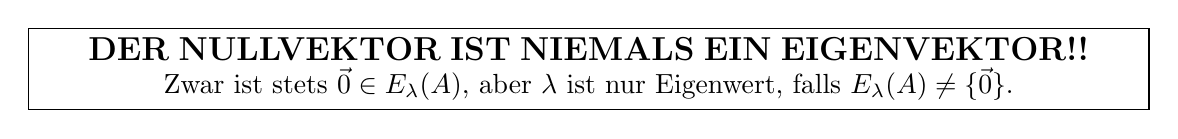
\begin{tikzpicture}
						\draw (0,0) node[draw, rectangle, text width=14cm,align=center]{\Umbruch{\textbf{\large DER NULLVEKTOR IST NIEMALS EIN EIGENVEKTOR!!} \normalsize Zwar ist stets $\vec{0}\in E_{\lambda}(A)$, aber $\lambda$ ist nur Eigenwert, falls $E_{\lambda}(A)\neq\{\vec{0}\}.$}};
					\end{tikzpicture}
				\end{center}
			\subsection{Definition: charakteristisches Polynom}
				\begin{itemize}
					\item $\chi_A(X):=det(X\1_n-A)\in\K[X]$ heißt \textbf{charakteristisches Polynom} von $A\in M_n(\K)$.
				\end{itemize}
			\subsection{Bemerkung: normiert}
				In der Literatur wird auch $\chi_A(X)=det(A-X\1)$ definiert. Die Definitionen unterscheiden sich um das Vorzeichen $(-1)^n$. Mit der zuvor gegebenen Definition ist $\chi_A(X)$ \textbf{normiert}, d.h. der Koeffizient des führenden Terms ist 1.
			\subsection{Lemma: Säkulargleichung}
				Sei $A\in M_n(\K)$ und $\lambda\in\K$
				\begin{enumerate}
					\item []
					\begin{enumerate}
						\item $E_{\lambda}(A)=LR(\lambda\1_n-A;\vec{0})\le\K^n.$
						\item []
						\item $\lambda$ ist Eigenwert von A $\Longleftrightarrow\chi_A(\lambda)=0$ (\textbf{Säkulargleichung}).
					\end{enumerate}
				\end{enumerate}
			\subsection{Definition Spur}
				\begin{itemize}
					\item Die \textbf{Spur} von $A\in M_n(\K)$ ist $Spur(A):=\sum^n_{i=1}A_{i,i}.$
				\end{itemize}
			\subsection{Lemma}
				Für $A\in M_n(\K))$ hat $\chi_A(X)$ die Gestalt:
				\begin{itemize}
					\item $\chi_A(X)=X^n-Spur(A)X^{n-1}+(\text{Terme vom Grad } n-2\ge r\ge1)+(-1)^ndet(A).$
				\end{itemize}
			\subsection{Guter Rat}
				Behalten Sie die während der Berechnung von $\chi_A(X)$ gefundenen Faktoren bei. Also \textit{NICHT} ausmultiplizieren, wenn es sich vermeiden lässt! Grund: Den Eigenwert kann man an den Faktoren leicht ablesen.
			\subsection{Hauptsatz der Algebra}
				\begin{itemize}
					\item $\forall p\in\C[X]$ mit $deg(p)=n$ und führendem Term $X^n:\exists\lambda_1,\dots,\lambda_n\in\C:p(X)=(X-\lambda_1)\cdot...\cdot(X-\lambda_n).$
				\end{itemize}
			\subsection{Definition, algb. Vielfachheit, geometrische Vielfachheit}
				Sei $A\in M_n(\K)$ und $\lambda\in\K$ ein Eigenwert von $A$.
				\begin{enumerate}
					\item []
					\begin{enumerate}
						\item $\lambda$ hat die \textbf{algebraische Vielfachheit} $k\in\N:\leftrightarrow\chi_A(X)$ wird von $(X-\lambda)^k$ ohne Rest geteilt, aber nicht von $(X-\lambda)^{k+1}.$
						\item []
						\item $dim(E_{\lambda}(A))$ heißt die \textbf{geometrische Vielfachheit} von $\lambda$.
					\end{enumerate}
				\end{enumerate}
			\subsection{Satz von Abel-Ruffini}
				Die Nullstellen eines Polynoms vom Grad $\ge$ 5 lassen sich im Allgemeinen nicht durch Grundrechenarten und Wurzelziehen berechnen. Dies gilt zum Beispiel für die Nullstelle $x=-1.1673...$ von $x^5-x+1$.
			\subsection{Tipps zur Nullstellensuche}
				Sei $f\in\R[X].$
				\begin{enumerate}
					\item []
					\begin{enumerate}
						\item Angenommen, die Koeffizienten von $f$ sind agnze Zahlen. \underline{Wenn} $f$ eine Nullstelle $\lambda\in\Z$ besitzt, so teilt $\lambda$ das Absolutglied von $f$. Auf diese Weise kann man ganzzahlige Nullstellen raten.
						\item []
						\item Kennt man eine Nullstelle $\lambda$ von $f$, so sind die restlichen Nullstellen von $f$ genau die Nullstellen von $\frac{f}{X-\lambda};$ die Polynomdivision feht ohne Rest auf (oder man hat einen Fehler gemacht).
						\item []
						\item Kennt man bereits eine Faktorisierung eines Polynoms, sollte man sie sich merken! Sind $g_1,g_2\in\R[X]$ vom Grad 2, so findet man die Nullstelle von $f=g_1g_2$ durch Anwendung der $p,q-Formel$ auf $g_1$ und $g_2$.
					\end{enumerate}					
				\end{enumerate}
\end{document}
